%  LaTeX support: latex@mdpi.com
%  In case you need support, please attach all files that are necessary for compiling as well as the log file, and specify the details of your LaTeX setup (which operating system and LaTeX version / tools you are using).

% You need to save the "mdpi.cls" and "mdpi.bst" files into the same folder as this template file.

%=================================================================
\documentclass[11pt,letterpaper]{article}

%\firstpage{1} 
%\makeatletter 
%\setcounter{page}{\@firstpage} 
%\makeatother 
%\articlenumber{x}
%------------------------------------------------------------------
% The following line should be uncommented if the LaTeX file is uploaded to arXiv.org
%\pdfoutput=1

%=================================================================
% Add packages and commands here. The following packages are loaded in our class file: fontenc, calc, indentfirst, fancyhdr, graphicx, lastpage, ifthen, lineno, float, amsmath, setspace, enumitem, mathpazo, booktabs, titlesec, etoolbox, amsthm, hyphenat, natbib, hyperref, footmisc, geometry, caption, url, mdframed

%=================================================================
%% Please use the following mathematics environments:

\usepackage{lineno}
\usepackage{setspace}
\usepackage{natbib}
\usepackage[capitalise,noabbrev]{cleveref}
\usepackage{rotating}
\usepackage{multirow}
\usepackage{tabularx}
\usepackage{adjustbox}
\usepackage{hyperref}
\usepackage[letterpaper, margin=1in]{geometry}

\RequirePackage[T1]{fontenc}
\RequirePackage[utf8]{inputenc}
\RequirePackage{calc}
\RequirePackage{indentfirst}
\RequirePackage{fancyhdr}
\RequirePackage{graphicx,epstopdf}
\RequirePackage{lastpage}
\RequirePackage{ifthen}
\RequirePackage{lineno}
\RequirePackage{float}
\RequirePackage{amsmath}
\RequirePackage{setspace}
\RequirePackage{enumitem}
\RequirePackage{mathpazo}
\RequirePackage{booktabs} % for \toprule etc. in tables
\RequirePackage[largestsep]{titlesec}
\RequirePackage{etoolbox} % for \AtBeginDocument


%=================================================================
% Full title of the paper (Capitalized)
\title{Climate Change and Curtailment: Evaluating Water Management Practices in the Context of Changing Runoff Regimes in a Snowmelt-Dominated Basin}

% Authors, for the paper (add full first names)
\author{Amy L. Steimke $^{1}$, Bangshuai Han $^{2}$, Jodi S. Brandt $^{3}$ and Alejandro N. Flores $^{1,}$* \\
$^{1}$ \quad Department of Geosciences, Boise State University, Boise, Idaho\\
$^{2}$ \quad Department of Geography, Ball State University, Muncie, Indiana\\
$^{3}$ \quad Human Environment Systems, Boise State University, Boise, Idaho\\
Correspondence: lejoflores@boisestate.edu}

% Contact information of the corresponding author
%\corres{Correspondence: lejoflores@boisestate.edu; Tel.: +1-208-426-2903}

% Current address and/or shared authorship
%\firstnote{Current address: Idaho Department of Environmental Quality, Boise, Idaho} 
%\secondnote{These authors contributed equally to this work.}

% Simple summary
%\simplesumm{}

% Abstract (Do not use inserted blank lines, i.e. \\) 
\begin{document}

\maketitle
\begin{center}
\MakeUppercase{This is a non-peer reviewed preprint submitted to} EarthArXiv
\end{center}

\linenumbers
\setstretch{1.8}

\section*{Abstract}
Climate change directly affects the hydrologic cycle in mountainous watersheds, which has consequences for downstream users. Improved water projections under diverse potential climate futures are critical to improving water security and management in these watersheds. The hydrologic science researchers and water resource managers, however, often focus on different metrics of flow regimes in changing climates. The research community tends to more closely focus on biophysical state and flux variables of the hydrologic system. Managers, meanwhile, tend to focus on key administrative benchmarks that govern the operation of complex water storage and distribution systems. Here, we examine potential hydrologic changes in a water supply basin in the western United States in the context of both biophysical states and fluxes, as well as from the perspective of how those changes map onto key variables that govern the administration of water resources in the region. The study site consists of the Upper Boise River Basin, ID. This snowmelt-dominated, mountainous watershed that supplies water to a semi-arid, agriculturally intensive and rapidly urbanizing region. Using the Envision integrated modeling framework, we created a hydrologic model and simulated hydrologic response to the year 2100 using six diverse climate scenarios. Annual discharge increased from historical values by an average of 13\% across all climate scenarios with a range of increase of 6-24\%, reflecting an increase in the precipitation in the climate projections.  Runoff timing was altered, with peak discharge occurring 4-33 days earlier and center of timing of streamflow occurring 4-17 days earlier by midcentury. Examining potential changes in the date junior water rights holders begin to be curtailed regionally (the Day of Allocation), we found that the Day of Allocation occurs up to 14 days earlier by 2100 across all climate scenarios, with one scenario suggesting this date could occur over a month earlier. These results suggest that current methods and policies of water rights accounting and management may need to be revised moving into the future.

% Keywords
\textbf{Keywords:} Climate Change; Runoff Regime; Snowmelt; Water Management; Water Rights; Day of Allocation; Flood Control; Water Supply

% The fields PACS, MSC, and JEL may be left empty or commented out if not applicable
%\PACS{J0101}
%\MSC{}
%\JEL{}

% If this is an expanded version of a conference paper, please cite it here: enter the full citation of your conference paper, and add $^\S$ in the end of the title of this article.
%\conference{}

%%%%%%%%%%%%%%%%%%%%%%%%%%%%%%%%%%%%%%%%%%
% Only for the journal Data:

%\dataset{DOI number or link to the deposited data set in cases where the data set is published or set to be published separately. If the data set is submitted and will be published as a supplement to this paper in the journal Data, this field will be filled by the editors of the journal. In this case, please make sure to submit the data set as a supplement when entering your manuscript into our manuscript editorial system.}

%\datasetlicense{license under which the data set is made available (CC0, CC-BY, CC-BY-SA, CC-BY-NC, etc.)}

%%%%%%%%%%%%%%%%%%%%%%%%%%%%%%%%%%%%%%%%%%



%\setcounter{section}{-1}

%% The [] brackets identify the author with the corresponding affiliation. 1, 2, 3, etc. should be inserted.

\section{Introduction}
Climate change exerts a significant control on global hydrologic regimes by influencing the timing, magnitude, phase, and seasonal variability in precipitation \citep{Mote:2005bv,Regonda:2005bl,Knowles:2006jc,Haddeland:2014kx}. Changes in temperature further influence how that precipitation moves through a watershed by affecting snowmelt timing, soil moisture, and evapotranspiration rates \citep{Barnett:2005ci,Li:2017jn}. While there is general consensus among scientists that the Earth is warming and will continue to do so, there remain significant uncertainties regarding the impacts of global warming on the water cycle and how those changes will be distributed regionally in the future \citep{Huntington:2006tl,Turral:2011uj}.

Significant changes in the water cycle can have serious consequences for water users and management across many sectors. It is estimated that more than two billion people currently live in highly water-stressed regions \citep{Oki:2006cu}, with this number projected to increase in the future \citep{Schewe:2014er}. Agriculture is vulnerable to changes in hydrologic regimes, especially in regions that rely on surface water resources for irrigation and in rain-fed systems \citep{Turral:2011uj}. Flooding could intensify, putting stress on current water management infrastructure as well as lessening the effectiveness of hydropower generation as runoff arrives earlier \citep{Markoff:2008tk}. Despite the seriousness of the potential impacts of hydrologic changes across sectors, the effectiveness of current water management systems, practices, and policies under changing hydrologic regimes is not well understood.

Many previous modeling studies have investigated how water resources will respond to climate change in snowmelt-dominated systems \citep{Adam:2009ie, Jin:2011ii, Ficklin:2013js, Gergel:2017vj}. However, results from such studies are not always presented in a way that is usable to water managers and users. Here we provide an example of how hydrologic modelers can generate results that may provide additional meaning for management decisions. Managers of these systems tend to focus on the ways in which climate variability and change will challenge existing water management protocols and practices. For example, in the American West, there are often hierarchies of water rights users who may be affected differently by projected changes in water availability \citep{Vicuna:2007gj}. Providing predictions more applicable to water users requires more in-depth and location-specific knowledge of water management and distribution but has the potential to provide more relevant information to a wider group of audiences. 

Snowmelt-dominated systems, particularly those in the western U.S., are especially vulnerable to climate change \citep{Barnett:2005ci,Stewart:2009jn,Li:2017jn}. Significant reservoirs, in the form of snow, develop at times (i.e., winter) and locations (i.e., high elevations) where that water cannot be used to grow crops and produce hydroelectricity. This snowpack at high elevations provides a natural reservoir that holds water in reserve and, ideally, slowly releases it into the spring and summer, into downstream agricultural areas. A complex system of water rights and management has been developed, and reservoir and canal systems engineered to store springtime runoff, mitigate flooding, and direct it to other locations when there is a demand for irrigation. This current system of water management infrastructure and protocols are set up to account for the historical range of hydrologic variability; however, it may not be adequate to adapt to future hydrologic regimes \citep{Palmer:2008dv}. With sufficient changes in the timing and magnitude of water delivery, as is projected with climate change, current management practices may be inadequate to meet the dual needs of flood control and late-season irrigation demand \citep{Barnett:2005ci}. However, it is uncertain to what extent current management practices may be stressed under future hydrologic regimes or when water management agencies can expect existing practices and policies to begin coming into conflict with the reality of altered runoff regimes. 

The overarching objective of this study is to better understand and quantify how climate change will impact future water resources and water management in the context of metrics that managers monitor and use to implement policy. We perform our study in the Upper Boise River Basin, ID, an ideal location because it is a relatively undisturbed high mountain watershed that is managed to provide water resources to an agriculturally-intensive and rapidly urbanizing region. We explore this connected biophysical and social system by combining a surface water hydrologic model with diverse climate projections to project potential changes in future regional hydrologic regimes. Furthermore, we translate our model outputs into a metric that is directly applicable to downstream water users and managers. Our specific research objectives are to:

\begin{enumerate}
\item Identify a range of climate projections and assess how they affect hydrologic parameters such as center of timing of streamflow, volume of annual water delivery, and snowpack levels through the end of the century; and
\item Identify how these changes in hydrologic regimes impact an associated metric that characterizes water storage and is used to enforce water rights accounting policies.
\end{enumerate}

What follows in this paper is: (1) a more detailed description of the study area, (2) an overview of our methodological approach, (3) results of this study, and (4) discussion, implications, and conclusions. 

\section{Methods}
\subsection{Study Area}
The Upper Boise River Basin (UBRB) is located in southwest Idaho (Figure \ref{fig:StudySite}) and supplies water for downstream users in the populated Boise metropolitan region. This watershed encompasses an area of 6,935 km${}^2$ with elevation ranging from approximately 930 to 3,000 m. It is bounded by the Sawtooth range in the east, the Payette River Basin to the north, and the Snake River Plain to the southwest. We delineated the study area by combining three Hydrologic Unit Code (HUC) 8 watersheds: the North and Middle Forks Boise (17050111), the South Fork Boise (17050113), and Boise-Mores (17050112). Due to the large variation in topography throughout the study area, regions shift from semi-arid grasslands and shrublands in the lowlands to coniferous forests in the highlands. In the UBRB, the dominant land covers are forest (43.0\%), shrubland (34.6\%) and grassland (20.9\%), with sparse human development within the watershed. The climate in this region is a continental Mediterranean climate (K\"{o}ppen \textit{Dsb}) with cold winters, warm summers, and the majority of precipitation falling in winter as snow. The overall average precipitation is $\sim$800 mm, with averages ranging from $\sim$400 mm at low elevations to over 1300 mm at high elevations \citep{Daly:2008hsa}.

The UBRB is the primary source of water for the downstream Treasure Valley region, which contains the state's three largest cities (Boise, Nampa, and Meridian) and roughly 40\% of the state's total population. The Treasure Valley is an agriculturally intensive region and contains approximately 1300 km${}^2$ of farmlands, many of which rely on irrigation water from the UBRB.  Like many other snowmelt-dominated watersheds in the West, the UBRB is heavily managed via three large storage reservoirs to fulfill the needs of flood control and downstream uses, especially for direct consumption in the Treasure Valley. Similar to other western states, water rights in this region follow the Prior Appropriation Doctrine, also known as "first in time – first in right." This doctrine states that the earliest beneficial users (i.e., senior water rights) retain their full water right, and those that came later (i.e., junior water rights) may retain their water rights as long as they do not infringe on those that came beforehand. As such, many junior water rights are curtailed during low water years, as total surface water rights in the Treasure Valley surpass 14,000 ft${}^3$/s, far exceeding the natural flow of the Boise River.

Previous studies indicate that the UBRB has already begun to respond hydrologically to climate change, noting an increase in summer streamflow temperatures \citep{Isaak:2010fn}, earlier timing of streamflow \citep{Clark:2010bq}, lengthened growing season \citep{Kunkel:2004bh}, and declining extreme low flow discharges \citep{Kormos:2016hy}. Additionally, there have been previous modeling studies that have used this basin to anticipate changes in hydrology under climate change \citep{Stillwater:2008uf,Jin:2011ii}. However, both of the aforementioned studies used an older generation of global climate models as their climate input and calibrated their models to streamflow alone. This study extends those previous works by making use of climate projections from the 5th Coupled Model Intercomparison Project \citep[CMIP5,][]{Taylor:2012jga}, calibrating the hydrologic model to multiple hydrologic metrics, and producing results that may provide additional meaning to water users.

\subsection{Modeling Framework}
Here we employ the Envision framework, a multiagent-based, spatially explicit modeling framework, to examine how regional hydrology may change with climate. Envision was created to examine relationships between human and natural environmental systems by integrating scenarios, data, and component models to assess regional landscape change \citep{Bolte:2007tb}. To this end, the modeling framework and software infrastructure of Envision support the integration of a variety of social and biophysical models in a spatiotemporally dynamic way. It is freely available and users can extend and enhance model capabilities by adding additional models as plugins. It has been extensively used recently in a wide variety of studies, from understanding urbanization impacts on streamflow \citep{Wu:2015tx} to projecting climate change impacts of land cover and land use \citep{Turner:2015wn}, and even to understand when fire occurrence and size is 'surprising' \citep{Hulse:2016wy}. Additionally, it has been used to integrate water rights to spatially allocate irrigation in the agriculturally intensive region below the UBRB \citep{Han:2017tx}. 

In this study, we use Envision version 6.197 and utilize the Flow extension to model future hydrology under various climate scenarios. In the following sections, we provide an overview of the modeling structure and the inputs needed for the various components.

\subsubsection{Spatial Coverage in Envision}

In Envision, the most refined spatial elements where model algorithms are applied are referred to as Integrated Decision Units (IDUs). The size and geometry of these polygons are dependent on the type of modeling being performed and the geospatial datasets required as input to those models. As such, there is no universally accepted method for creating IDU coverage. In this study, we used three datasets to form the IDU geometry: surface management agency, land cover, and HUC 12 stream catchments (Table \ref{table:DataSources}). As such, the IDU coverage will preserve boundaries between HUC 12 catchments, cognizant land management agencies, as well as boundaries between vegetation classes.  

The datasets were processed in ArcMap 10.1. To shorten Envision's computation time, we coarsened the land cover dataset from 30 to 100 m in increments of 10 m. We used a nearest neighbor algorithm to resample land cover types to more accurately capture the original distribution of coverage in the land cover dataset. The other two datasets were polygon geospatial datasets that required very little processing besides renaming attributes to be consistent with the Envision framework requirements.

We created our IDU coverage by intersecting the three aforementioned datasets, creating 31,625 polygons. We extracted the average elevation for each IDU and also assigned an elevation class from 1-4, corresponding to 0-1500, 1500-2000, 2000-2500, and >2500 meters to allow binning and analysis of results by elevation band. Additionally, to aid in analysis and querying we created a three-tiered hierarchy of land cover classification ranging from general (e.g. Natural Vegetation) to more specific (e.g. Evergreen Forest), which was formed by grouping NLCD classifications that are similar (Figure \ref{fig:LULCtree}).

The hydrologic model in Envision applies algorithms to Hydrologic Response Units \citep[HRUs,][]{Jin:2011ii,Turner:2016ia}, which are an aggregation of IDUs that would theoretically behave hydrologically similar. To create the HRU coverage, we grouped polygons that had the same intermediate land cover (Figure \ref{fig:LULCtree}), identical elevation class, and were located in the same HUC-12 catchment. This resulted in 9,465 HRUs.

\subsubsection{Hydrologic System Model}

An extension in Envision called Flow provides flexibility in modeling hydrology and the use of different model representations of hydrologic processes. In this study, we used a modified version of the HBV (Hydrologiska Byr\r{a}ns Vattenbalansavdelning) rainfall-runoff model \citep{Bergstrom:1976tr} for surface hydrology. HBV is a commonly used conceptual model \citep{Seibert:2000wi,Woodsmith:2007vz,Abebe:2010to,Bergstrom:2015ck} but has been modified by Envision’s developers to be spatially distributed. Each HRU is conceptualized as a linked reservoir with five layers of storage: snowpack, lakes, soil, upper groundwater, and lower groundwater (Figure \ref{fig:ModelFlowchart}). Runoff from each HRU is routed to streams using HUC12 flowlines from NHDplus V2 (Table \ref{table:DataSources}). The water balance in Flow is described by the following equation:

\begin{equation}
P - ET - Q = \frac{d}{dt}\left[SP + SM + UZ + LZ + lakes\right]
\end{equation}

where $P$ is precipitation [mm/d], $ET$ is evapotranspiration [mm/d], $Q$ is runoff [mm/d], $SP$ is snow storage [mm], $SM$ is soil moisture storage [mm], $UZ$ is upper groundwater storage [mm], $LZ$ is lower groundwater storage [mm], and $lakes$ refers to lake storage [mm]. A more thorough description of the HBV model can be found in other papers \citep{Seibert:1999vg,Bergstrom:2015ck} and a more detailed description of Flow can be found on Envision’s website (\href{http://envision.bioe.orst.edu/}{http://envision.bioe.orst.edu/}).

Evapotranspiration (ET) is calculated via a modified Penman-Monteith approach described in the Food and Agriculture Organization’s Irrigation and Drainage paper 56 (FAO56) where a crop coefficient is applied to the ET of a reference plant \citep{Allen:vn} and was later developed specifically for Idaho \citep{Allen:2007ta} using the following equation:

\begin{equation}
ET = ET_r \cdot K_c
\end{equation}

where $ET$ = evapotranspiration, $ET_r$ = reference evapotranspiration (alfalfa, for Idaho), and $K_c$ = crop coefficient.

We used this equation and applied crop coefficient curves that either matched our land cover type directly or estimated crop coefficient curves based upon similarities of crops to land cover types (Table \ref{table:LandCoverType}). Crop coefficients were obtained from AgriMet and \citep{Allen:2007ta}, with a few modified land cover coefficients from \citep{Inouye:2014ws}.  

\subsection{Climate Inputs}

We used statistically downscaled climate data using the MACA (Multivariate Adaptive Constructed Analogs) method version 1.0 for both historic and future simulations \citep{Abatzoglou:2011kca}. This data has a spatial resolution of 4 km across the continental U.S. and is available daily for 1950-2100. Downscaled data is available for 20 Global Climate Models (GCMs) from CMIP5 for both Representative Concentration Pathway (RCP) 4.5 and 8.5 scenarios. RCPs are a consistent set of projections that are named according to their additional radiating forcing level at 2100, such that RCP 4.5 equates to +4.5 W/m${}^2$ radiative forcing relative to pre-industrial values by the end of the century \citep{vanVuuren:2011tu}. 

For future simulations, we selected GCMs based upon two criteria. First, we halved our GCM selection to models that performed relatively well when ran over the historical period in the Pacific Northwest region \citep{Rupp:2013ea}, meaning they produced less relative error when compared across several metrics. Secondly, we selected GCMs that captured the range of variability between models as it related to changes in precipitation and temperature (Figure \ref{fig:ClimateChange}). We selected three climate models: CanESM2 (hotter, wetter), CNRM-CM5 (warmer, slightly wetter), and GFDL-ESM2M (less warm, drier), and ran each one for RCP 4.5 and 8.5 scenarios, which resulted in six total future climate scenarios (Figure \ref{fig:ClimateChangeSelected}). Table \ref{table:ExperimentDesign} provides a naming convention for these six future climate scenarios to ease in discussing results and implications. For historical simulations from 1980-2014, we used a historical climate dataset, METDATA \citep{Abatzoglou:2011em}, which was developed using data from the North American Land Data Assimilation System Phase 2 \citep[NLDAS-2,][]{Mitchell:2004hf} and from the Parameter-elevation Regressions on Independent Slopes Model \citep[PRISM,][]{Daly:2008hsa}.  

The downscaled variables Envision requires for Flow are daily maximum, minimum, and average temperature, precipitation amount, specific humidity, daily downward shortwave radiation, and wind speed. To format the variables for Envision, the following procedure was followed: (1) subset data to the specified region, (2) convert units and rename variables where needed, (3) compute average temperature as the average between minimum and maximum temperature, (4) calculate overall wind speed from the eastward and northward components provided by MACA, and (5) subset into annual files. Scripts created for pre-processing MACA climate data are available online at \href{https://github.com/asteimke/MACA\_EnvisionClimate}{https://github.com/asteimke/MACA\_EnvisionClimate}.

\subsection{Calibration and Validation}

HBV is a semi-conceptual model, and as such, parameters required as input to the model are obtained through calibration because most parameters cannot be physically measured \citep{Bergstrom:2015ck}. Numerous combinations of parameter values can yield equally good results \citep[i.e. the equifinality issue,][]{Beven:2006wa,Gupta:2005wl}, which makes it difficult to select the best parameter set. To combat this issue, some studies \citep{Madsen:2003un,Inouye:2014ws} build an objective function to find an adequate parameter set based on the type of information they want to yield from the model (e.g. streamflow volume, timing, snowpack, etc.). Typically, the calibration-validation procedure takes the form of a data-denial experiment. The model is run over a calibration period to select best parameter sets and then re-run over a validation period to ensure that the selected parameter set performs well during this period for which data was not used to calibrate the model.

Fourteen parameters are included within the HBV model and govern rates of exchange between reservoirs. We held five of them constant, while the remaining nine were calibrated. $CFR$ and $CWH$ are insensitive parameters and were held constant as is often done in HBV applications \citep{Seibert:1997vw}. While many of the parameters are conceptual and cannot be measured, three of them are based on physical properties, so we fixed those parameters to better represent the reality of our study area. We used the Global Gridded Surfaces of Selected Soil Characteristics (IGBP-DIS) dataset \citep{Hope:1994wq} and took the average of values for the study area. We used the following datasets from IGBP-DIS: soil field capacity, soil profile available water capacity, and soil wilting point for the parameters $FC$, $LP$, and $WP$, respectively (Table \ref{table:FlowParams}). In each model run, we randomly selected the remaining nine parameters from a uniform distribution between ranges of possible values (Table \ref{table:FlowParams}) defined based on previous studies \citep{Inouye:2014ws,Han:2017tx}. 

We ran the model for 1000 simulations at a daily time step over the years 1988-2000 (12 years + 1 spin-up year). We selected this time interval for calibration because it encompasses a reasonably long time period and includes both wet and dry years. We compared model output to historical stream discharge records from three long-term USGS gaging stations and snowpack observations from nine SNOTEL (SNOw TELemetry) stations, omitting all leap days from these datasets (Table \ref{table:CalValData}). For each run, we calculated the Nash-Sutcliffe Efficiency \citep[$NSE$,][]{Nash:1970vw}, $\log NSE$, and a volume error ($VE$) using the following equations:

\begin{equation}
NSE = 1 - \frac{\sum_{t=1}^{T} \left(Q_{obs}^t - Q_{sim}^t\right)^2}{\sum_{t=1}^{T} \left(Q_{obs}^t - \overline{Q_{obs}}\right)^2}
\end{equation}

\begin{equation}
\log NSE = 1 - \frac{\sum_{t=1}^{T} \left(\ln{Q_{obs}^t} - \ln{Q_{sim}^t}\right)^2}{\sum_{t=1}^{T} \left(\ln{Q_{obs}^t} - \ln{\overline{Q_{obs}}}\right)^2}
\end{equation}

\begin{equation}
VE = \frac{\sum_{t=1}^{t} \left(Q_{obs}^t - Q_{sim}^t\right)}{\sum_{t=1}^{t} \left(Q_{obs}^t\right)}
\end{equation}

where $Q_{obs}$ is the observed value and $Q_{sim}$ is the simulated value at each daily time step.

NSE coefficients range from $-\infty$ to 1, with 1 indicating a perfect fit of the model to the observed data, and a value of $NSE$ > 0 indicating the model is a better predictor than the historically observed mean. Typically, a model is deemed satisfactory if the $NSE$ is larger than 0.5 \citep{NMoriasi:2007tj}. The logarithmic form of the $NSE$ also ranges from $-\infty$ to 1, but is more sensitive to low flow and still reacts to peak flows \citep{krause:hal-00296842}. The volume error provides insight into whether the model overestimates ($VE$<0) or underestimates ($VE$>0) total volume, with a value closest to 0 being ideal.

We created an objective function to select the best-performing parameter set and was developed based on work by \citep{Inouye:2014ws}:

\begin{equation}
Obj = \frac{1}{3}\left(NSE_G\right) + \frac{1}{3}\left(logNSE_G\right) + \frac{1}{3}\left(NSE_S\right) - 0.2\cdot\left|VE_G\right|
\end{equation}

where $NSE_G$ is the Nash-Sutcliffe Coefficient of discharge weighted by an areal average of the gauges, $VE_G$  is the volume error for the gauges weighted by an areal average, and $NSE_S$ is the averaged Nash-Sutcliffe Coefficient for SWE (snow water equivalent) for all SNOTEL sites. 

The objective function ideally is as close to 1 as possible, as we wish to maximize $NSE$ and minimize volume bias. The top 1\% best performing parameter sets were run over the eight-year validation period (2001-2008) and the set that performed on average the best in both calibration and validation years was chosen for our model. Results of the calibration/validation exercises are reported in the Results section of this manuscript.

\subsection{Evaluating Climate Change Impacts}

To assess the potential impact of climate change on hydrologic regimes, we examined three broad metrics: streamflow, snowpack, and water management. A more detailed description of methods for these metrics is described here.

\subsubsection{Streamflow}
While Envision has the capability to examine discharge values anywhere along its stream network, we focused here on the aggregation of streamflows for the basin. In all cases, unless mentioned otherwise, streamflow results are for the unregulated discharge on the Boise River occurring at the location of Lucky Peak Dam's outlet, i.e. the pourpoint of the watershed (Figure \ref{fig:StudySite}). This modeled streamflow, as well as daily values for the three major tributaries, can be obtained online \citep{Steimke:2017hb}. 

To assess climate change impacts on streamflow, we looked at changes in the amount and timing of discharge. An additional metric we used was the center of timing (CT) of streamflow, which is the date when half of the annual volume of water during the water year has arrived at a specified location. We calculated the CT for historical data and future simulations with the following equation \citep{Stewart:2005ed}: 

\begin{equation}
CT = \frac{\sum \left(t_iQ_i\right)}{\sum Q_i}
\end{equation}

where $t_i$ is the time in days from the start of the water year (October 1) and $Q_i$ is the discharge for that date. 

\subsubsection{Snowpack}

To assess climate impacts on the basin’s snowpack, we looked at averaged values over three elevation zones: low (1500-2000 m), medium (2000-2500 m), and high (2500+ m) zones. These zones cover 43.4\%, 25.8\%, and 6.9\% of the area of interest, respectively. We do not show results for elevations less than 1500 m as the lowest SNOTEL station to aid in calibration is the Prairie site at 1463 m. Within these three zones, we examine the dates and magnitudes of when SWE is at its maximum, as well the April 1 SWE amount. Water managers have historically used the amount of SWE on this date as an indicator for water availability in the upcoming year, as it has correlated well with maximum SWE at many SNOTEL sites in the West historically \citep{Bohr:2001bc}.

\subsubsection{Water Management}

Since 1986, water managers annually declare a Day of Allocation (DOA) in the Lower Boise River Basin for the purpose of water rights accounting during the irrigation season (April – October). This day is declared on or after the date of maximum reservoir fill and once natural flow is less than irrigation demand (Memo from IDWR Technical Hydrologist Liz Cresto to IDWR Director Gary Spackman, November 4, 2014, Subject: Accounting for the distribution of water to the federal on-stream reservoirs in Water District 63). The DOA occurs after peak runoff and has been shown historically to typically occur once the natural flow of the Boise River at Lucky Peak reaches below 4000 ft${}^3$/s \citep{Garst:2017bg}, or 113.3 m${}^3$/s (Figure \ref{fig:DayOfAllocation}), which is roughly equivalent to the diversion demand of the river. It is beneficial for farmers if the DOA occurs later in the season because after the DOA is declared water rights begin to be curtailed, starting with the junior-most water rights holders. While the term DOA is unique to three major river basins in Idaho (i.e. Boise, Payette, and Upper Snake river basins), many western states have similar methods for appropriating water as the irrigation season begins.

To predict how the DOA may change in our modeled scenarios, we assume that diversion rights will continue to be approximately 113.3 m${}^3$/s. We model our DOA date by finding the last day during peak runoff during the irrigation season that flow is greater than 113.3 m${}^3$/s and select the day after. We then manually observe the hydrographs and the DOA selected to ensure we are capturing a date on the downfalling limb of peak runoff and not a later season event. If a later season event was modeled, then we manually select the date on which modeled flow falls below 113.3 m${}^3$/s during the recession limb of spring runoff. We ran the model during the historical period to investigate how well the model reproduces historical DOA using this definition, which provides confidence in our interpretation of DOA changes in modeled future scenarios.

\section{Results}

\subsection{Calibration and Validation}
We calibrated and validated the model using historical records from three USGS gauges and nine SNOTEL sites. The parameter set that performed best had an objective function score of 0.63 and 0.62 for calibration and validation periods, respectively (Table \ref{table:CalValValues}). We averaged the NSE for each gauge by its respective drainage area, which resulted in a $NSE$ of 0.71 and 0.70 for calibration and validation, respectively. However, it should be noted that Mores Creek on its own achieved a lesser NSE of 0.58, which is potentially due to this smaller watershed exhibiting some major differences from the other two (notably lower elevation, less precipitation, and less steepness).

Among all gauges, we see relatively good agreement between the model simulations and observed flow for the historic period (Figure \ref{fig:CalVal}), although the model frequently under predicts the magnitude of peak flows at all gauge sites and over predicts baseflow at Mores Creek. While the unregulated flow for the Boise River at Lucky Peak (Table \ref{table:CalValData}) was not used to calibrate the model, we used this as an additional verification dataset to ensure accuracy of the model. With the chosen parameter set, we achieved a NSE at this site of 0.74 and VE of -0.01 averaged over the entire calibration and validation period, providing additional confidence in our model.

\subsection{Streamflow}

\subsubsection{Annual Discharge}

In all future climate scenarios, we see an increase in the median annual discharge from the Boise River (Figure \ref{fig:BoxPlotDischarge}). By midcentury (2040-2069), all climate scenarios showed an increase in annual discharge over historical (1950-2009) averages, with an average increase of 13\% and ranges of increase from 6-24\%. RCP 8.5 climate scenarios showed a greater rate of increase over RCP 4.5 scenarios. Because our hydrologic model did not perform well historically in accurately capturing the magnitude of peak discharges, we do not have adequate confidence to predict future magnitudes in peak or low flows. 

\subsubsection{Timing of Discharge}

While we see some changes in the volume of annual discharge, streamflow is also projected to arrive at significantly different times than in the historical past. However, these arrival times vary greatly between different climate models.

In most future climate scenarios, the date of peak discharge occurs earlier in the season, with an increase in early winter flooding events (Figure \ref{fig:PeakDischargeDate}). In extreme climate cases (i.e. C-85), the average peak discharge occurs approximately 45 days earlier in the period 2040-2060 relative to 1980-2009. In a conservative climate model (i.e. A-45), peak discharge may only be on average about 5 days earlier by midcentury. 

To get an understanding of the shift in seasonality and variance between climate scenarios, we can look at the multi-decadal averaged hydrographs between two endmember climate models predicting the least and most amount of change from historical averages (Figure \ref{fig:HydrographDecadeAvg}). With the coolest climate scenario (A-45), there is little discernible deviation from the historical average hydrograph. However, if we look at the warmest climate scenario (C-85), we see obvious differences in the average hydrograph, where by 2050-2070 the average peak of the hydrograph is over a month and a half earlier. Overall, this warmest scenario shows a shift in seasonality through time, where we see flows occurring earlier in the season with an additional increase in early-season, mid-winter discharge events.

\subsubsection{Center of Timing}

The historical average (1980-2009) center of timing (CT) of streamflow for the UBRB is April 22. In our simulations, we see this date shift earlier in most of our climate scenarios (Figure \ref{fig:CenterOfTiming}). Three scenarios (C-45, B-45, and A-85) behave similarly and begin deviating from the historical range of variability between 2040 and 2050, showing a CT date that is 13-17 days earlier on average between 2070 and 2099. Both C-85 and B-85 begin to deviate from historical averages around 2030 and exhibit an average a CT date 27-30 days earlier than the historical average during the 2070-2099 period. A-45 remains relatively similar to historical ranges through the century, although its CT date shifts a few days earlier, resulting in fewer occurrences of exceeding the historical 75th percentile of CT date. 

\subsection{Snowpack}

\subsubsection{April 1 SWE}

Our results (Figure \ref{fig:PercentApril1SWE}) show a substantial decrease in April 1 SWE in five of the climate scenarios, with lower elevations essentially experiencing no April 1 SWE by midcentury. Higher elevations remain less affected across all RCP 4.5 scenarios but begin substantially decreasing around 2050 in B-85 and C-85 where they experience virtually no April 1 SWE from 2080-2100. Under the A-45 scenario, April 1 SWE experiences variability, but has no discernible downward trend. 

\subsubsection{Dates and amounts of maximum SWE}

The previous section suggests that April 1 SWE will, at some point in the future, cease to be a good indicator of maximum SWE. In terms of evaluating potential climate change impacts on SWE in the context of water supply, therefore, it is necessary to examine additional metrics. Specifically, we see the date of maximum SWE happening earlier across most scenarios (Figure \ref{fig:MaxSWEDate}). Both C-85 and B-85 show maximum SWE occurring more than two months earlier on average by the end of the century. Three scenarios, A-85, C-45, and B-45 behave similarly with maximum SWE date happening between 38 and 42 days earlier than historically observed averages. A-45 produces little change in timing by the end of the century (7 days earlier on average). 

The magnitudes of maximum SWE may change as well (Figure \ref{fig:MaxSWEMidElev}). Within mid-elevation zones (2000-2500 m), we see a drastic decrease in the occurrence of annual amounts above the historical 75${}^\textrm{th}$ percentile in five of our climate scenarios. Furthermore, from 2050 onward, we see that 80\% (C-85) and 84\% (B-85) of the time the maximum SWE is falling below the historical 25${}^\textrm{th}$ percentile. As with many of the metrics previously mentioned, A-45 shows very little change from historical trends.

\subsection{Water Management}

\subsubsection{Day of Allocation}

The developed model reasonably reproduces the DOA in the historical period (R${}^2$=0.90), although it over-predicted the date on average 4.8 days later (Figure \ref{fig:DayOfAllocation}). Thus, the defined metric for the DOA provides a reasonably robust vehicle to analyze how the DOA may shift under different climate scenarios.
Our results show the DOA occurring much earlier under four of our scenarios (Figure \ref{fig:FutureDayOfAllocation}), ranging from 11 to 33 days earlier on average by the end of the century. Scenarios A-45 and B-45 resulted in little to no change in the trend of DOA. While the DOA remains variable on an interannual basis, we do not see significant changes in variability of DOA through time (Table \ref{table:SimulatedDOA}).

\section{Discussion}

\subsection{Trends in Future Hydrologic Regimes}

We calibrated our model using metrics that included historic snowpack levels, daily streamflow, logarithmic transformation of streamflow, and streamflow volume. Choosing multiple metrics to select the best parameter set provides some additional confidence that the model is simulating key attributes of historical hydrologic regimes and, therefore, strengthens confidence in the robustness of our interpretations of future climate change impacts on hydrologic regimes predicted by the model. 

We have shown that a variety of hydrologic regime characteristics within the UBRB could exhibit significant changes, depending on which climate model and RCP scenario is used. However, certain trends are consistent across several considered climate scenarios and are consistent with other projections \citep{Adam:2009ie,Inouye:2014ws,Gergel:2017vj}. Our results suggest an increase in annual water discharge, but with significantly altered timing, with flows arriving much earlier than historically. Our modeled results also show a decrease in the total amount of snowpack, an earlier melting date, and earlier dates of peak snowpack. In order to reconcile how annual discharge can increase while the snowpack is consistently smaller in volume and more ephemeral in time, we examined the seasonality of the precipitation input to the model. This allows us to better understand whether observed changes in discharge volume are primarily related to changes in the seasonality of input precipitation, changes in the seasonal dynamics of snowpacks, or some combination of both. Typically, however, the precipitation exhibits increases across all seasons rather than large shifts between seasons in precipitation. Accordingly, this may indicate that the basin could begin transitioning from being snowmelt-dominated to a regime that is mixed rain- and snow-dominated watershed moving forward.

\subsection{Management Implications}

Our modeled scenarios support previous studies \citep{Pederson:2011ep,Klos:2014jra} that April 1 SWE is not likely to remain a reliable metric for estimating maximum SWE (and therefore snow water storage) in the future for water resource prediction and management. This work suggests declines in the amount of SWE on April 1 and a maximum SWE date over a month earlier than historically observed in five of the six considered scenarios. Rather than choosing a static date to estimate peak SWE across a vast region, managers may need to more closely monitor the relationship between hydrologic regimes and the timing of peak SWE in their regions, potentially necessitating increased investment in monitoring and modeling of snow conditions.

There is little evidence to conclude that we will experience future water shortages from the UBRB in an absolute sense, as most models suggest at least a small increase in annual discharge. However, we will likely experience hydrologic shifts that are outside of our current range of variability. All climate scenarios show peak discharge occurring earlier in the year. This is problematic for reservoir managers who primarily manage dams to provide storage for flood mitigation. Managers might have to release more 'usable' water from reservoirs in preparation for these events, which potentially could equate to shortages later in the irrigation season. Such outcomes could be viewed as an "operational deficit" that arises because of a mismatch between the release of water from storage for flood mitigation and the timing of water allocation as codified in water rights laws.

At the same time, in this region agricultural land is increasingly transitioning to urban areas \citep{Dahal:2017ux}, which could indicate that future water demand may be substantially different from the past. With warmer climates, farmers might plant earlier in the season, which would change the timing of water demand. Recent modeling efforts have shown that current water rights are not always able to support irrigation demand \citep{Han:2017tx}. Agricultural water use efficiency, however, is likely to increase with technological advances like genetically modified crops, which could change spatiotemporal patterns of water demand. A more comprehensive examination of how, when, and where water is being used downstream and how that may change in the future will help managers understand to what extent regional water infrastructure is vulnerable and the potential policies that might help to mitigate effects. 

Our results show that under most climate scenarios, the Day of Allocation occurs much earlier than it has historically, with two models showing the date moving by over a month earlier. If this projection becomes reality, then there is an earnest need for exploring potential conflicts between water users in the future as curtailments may come increasingly early and impact more water rights holders than in previous decades. It may be necessary, for instance, to incentivize farmers to transition to more efficient irrigation practices (e.g. switching from flood to drip irrigation) and to diversify with crops that require less water, or expand other solutions like water banking and water markets. If junior water rights holders are curtailed over a month earlier without any mitigation practices set in place, it may result in substantial repercussions to Idaho’s agricultural sector. These effects are compounded if other mountain water supply basins exhibit similar changes to hydrologic regimes. 

\subsection{Study Limitations}

It is worth noting that this study did not simulate reservoir operations. There are three dams present in the study area that are located close to the outlet of the basin. For purposes of simplicity, the present work focuses on evaluating the ramifications of climate change on natural flows in the UBRB and capturing reservoir operations is outside the scope of this study. A significant challenge in future work will arise from the need to develop plausible scenarios by which water managers from federal agencies, irrigation districts, environmental groups, and utility companies can create strategies to adapt to potential changes in hydrologic regimes similar to those simulated here. Given the complexities in both biophysical and social responses to climate change, such studies will likely need to be region- and context-specific.  

An additional source of uncertainty in this study lies in the land cover data used in the hydrologic model, which was treated as static. Specifically, the land cover dataset used represents a snapshot estimated based on Landsat reflectances from 2011. Vegetation along ecotones is sensitive to changes in climate, and there are likely to be additional large-scale vegetation and land cover changes that occur after wildfire events or through land management actions. Future modeling studies should incorporate plausible shifts in vegetation to understand the sensitivity of changes in hydrologic regimes to associated changes in land cover as well as climate change. This might be best accomplished using a physically-based model, rather than the conceptual model used in this study, to be able to better capture complex interactions between climate, hydrology, vegetation dynamics, and changing land cover.


\subsection{Conclusions}

In this study, we used an integrated modeling framework, Envision, to simulate future hydrology in a mountainous watershed that supports an urban and agriculturally intensive region below it. We calibrated the hydrologic model to metrics of both streamflow and snowpack, and it performed well under historical conditions. We ran the model to the year 2100 under six climate scenarios (three GCMs and two RCP scenarios) to analyze future possible hydrologic regimes. 

Our results suggest that overall annual streamflow will increase, and five of six scenarios suggest hydrologic regimes that will deliver runoff substantially earlier than historically observed. This could lead to operational water shortages later in the season as water managers balance release of water from storage in reservoirs to mitigate flooding hazards with retention of water for supplying irrigation in the warm, dry summers. Without changes in existing policies, these hydrologic regimes could have repercussions to late-season irrigation demand, hydropower operations, recreational flows, and municipal water supply. 

Mountainous, snowmelt-dominated watersheds have already begun responding to climate change, which will almost certainly continue in the future. The degree to which the runoff response of these watersheds changes in association with climate change is uncertain, and will depend heavily on the nature of the change in the climatic forcing variables. Increasingly sophisticated comparisons with climate model predictions and observations, as well as regionally focused and contextual modeling of coupled hydrologic and social systems, will improve our ability to constrain how hydrologic regimes will change in the future. This may increase the efficacy of efforts to respond to changes and potential conflicts between potentially competing demands for water.

\section*{Acknowledgments}
This study was made possible with funding support from NSF CAREER award EAR-1352631, and NSF Established Program to Stimulate Competitive Research award IIA-1301792.

%% REFERENCES

%% The reference list is compiled as follows:
\renewcommand\bibname{References}
\bibliographystyle{mdpi}
\bibliography{Steimke_etal_2018-REFs}
%%
%% URLs and DOIs can be entered in your BibTeX file as:
%%
%% URL = {http://www.xyz.org/~jones/idx_g.htm}
%% DOI = {10.5194/xyz}


%% LITERATURE CITATIONS
%%
%% command                        & example result
%% \citet{jones90}|               & Jones et al. (1990)
%% \citep{jones90}|               & (Jones et al., 1990)
%% \citep{jones90,jones93}|       & (Jones et al., 1990, 1993)
%% \citep[p.~32]{jones90}|        & (Jones et al., 1990, p.~32)
%% \citep[e.g.,][]{jones90}|      & (e.g., Jones et al., 1990)
%% \citep[e.g.,][p.~32]{jones90}| & (e.g., Jones et al., 1990, p.~32)
%% \citeauthor{jones90}|          & Jones et al.
%% \citeyear{jones90}|            & 1990



%% FIGURES

%% When figures and tables are placed at the end of the MS (article in one-column style), please add \clearpage
%% between bibliography and first table and/or figure as well as between each table and/or figure.


%% ONE-COLUMN FIGURES
\clearpage

\begin{figure}
\centering
\includegraphics[width=\textwidth]{figure-files/figure1.png}
\caption{Overview of the study area with major land cover types and locations of SNOTEL stations and gauge locations (see Table \ref{table:CalValData} for names of gauges).}
\label{fig:StudySite}
\end{figure}
\clearpage

\begin{figure}
\centering
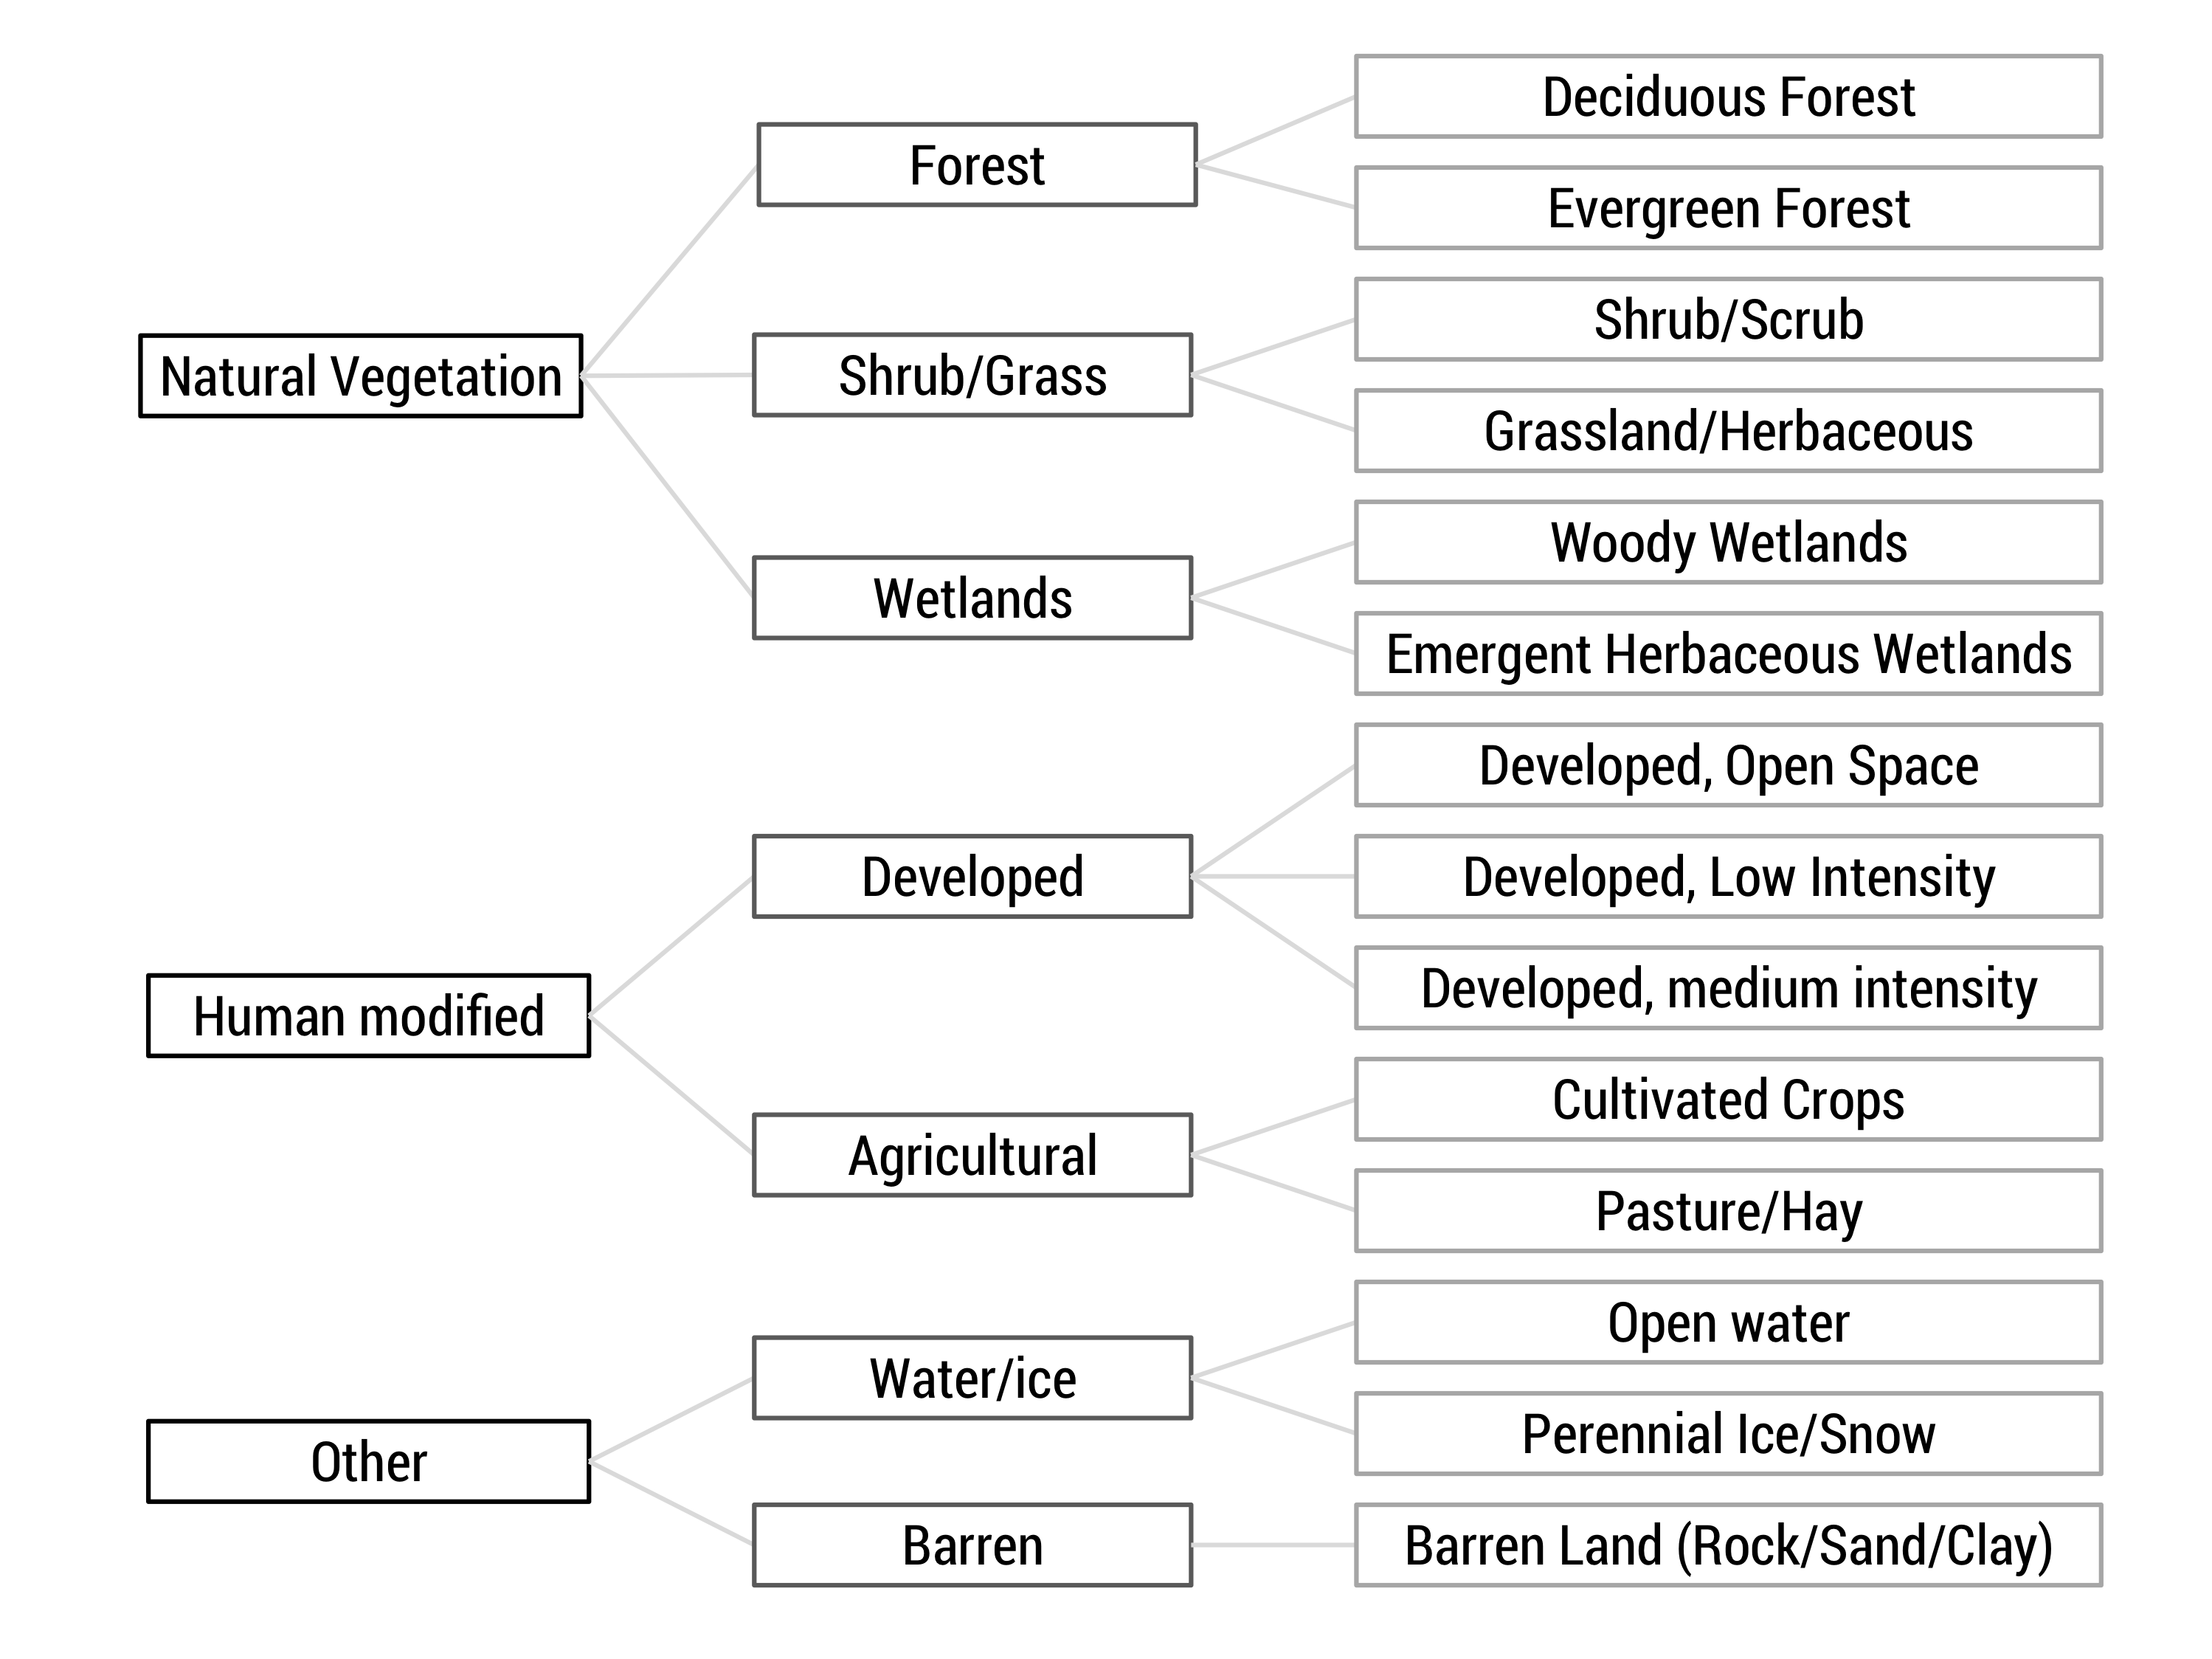
\includegraphics[width=\textwidth]{figure-files/figure2.png}
\caption{Land use/land cover tree developed for Envision. The tree allows for modeling algorithms to be applied at different hierarchy levels, from more general to more specific land types. The finest categories on the right correspond to the NLCD land classification system.}
\label{fig:LULCtree}
\end{figure}
\clearpage

\begin{figure}
\centering
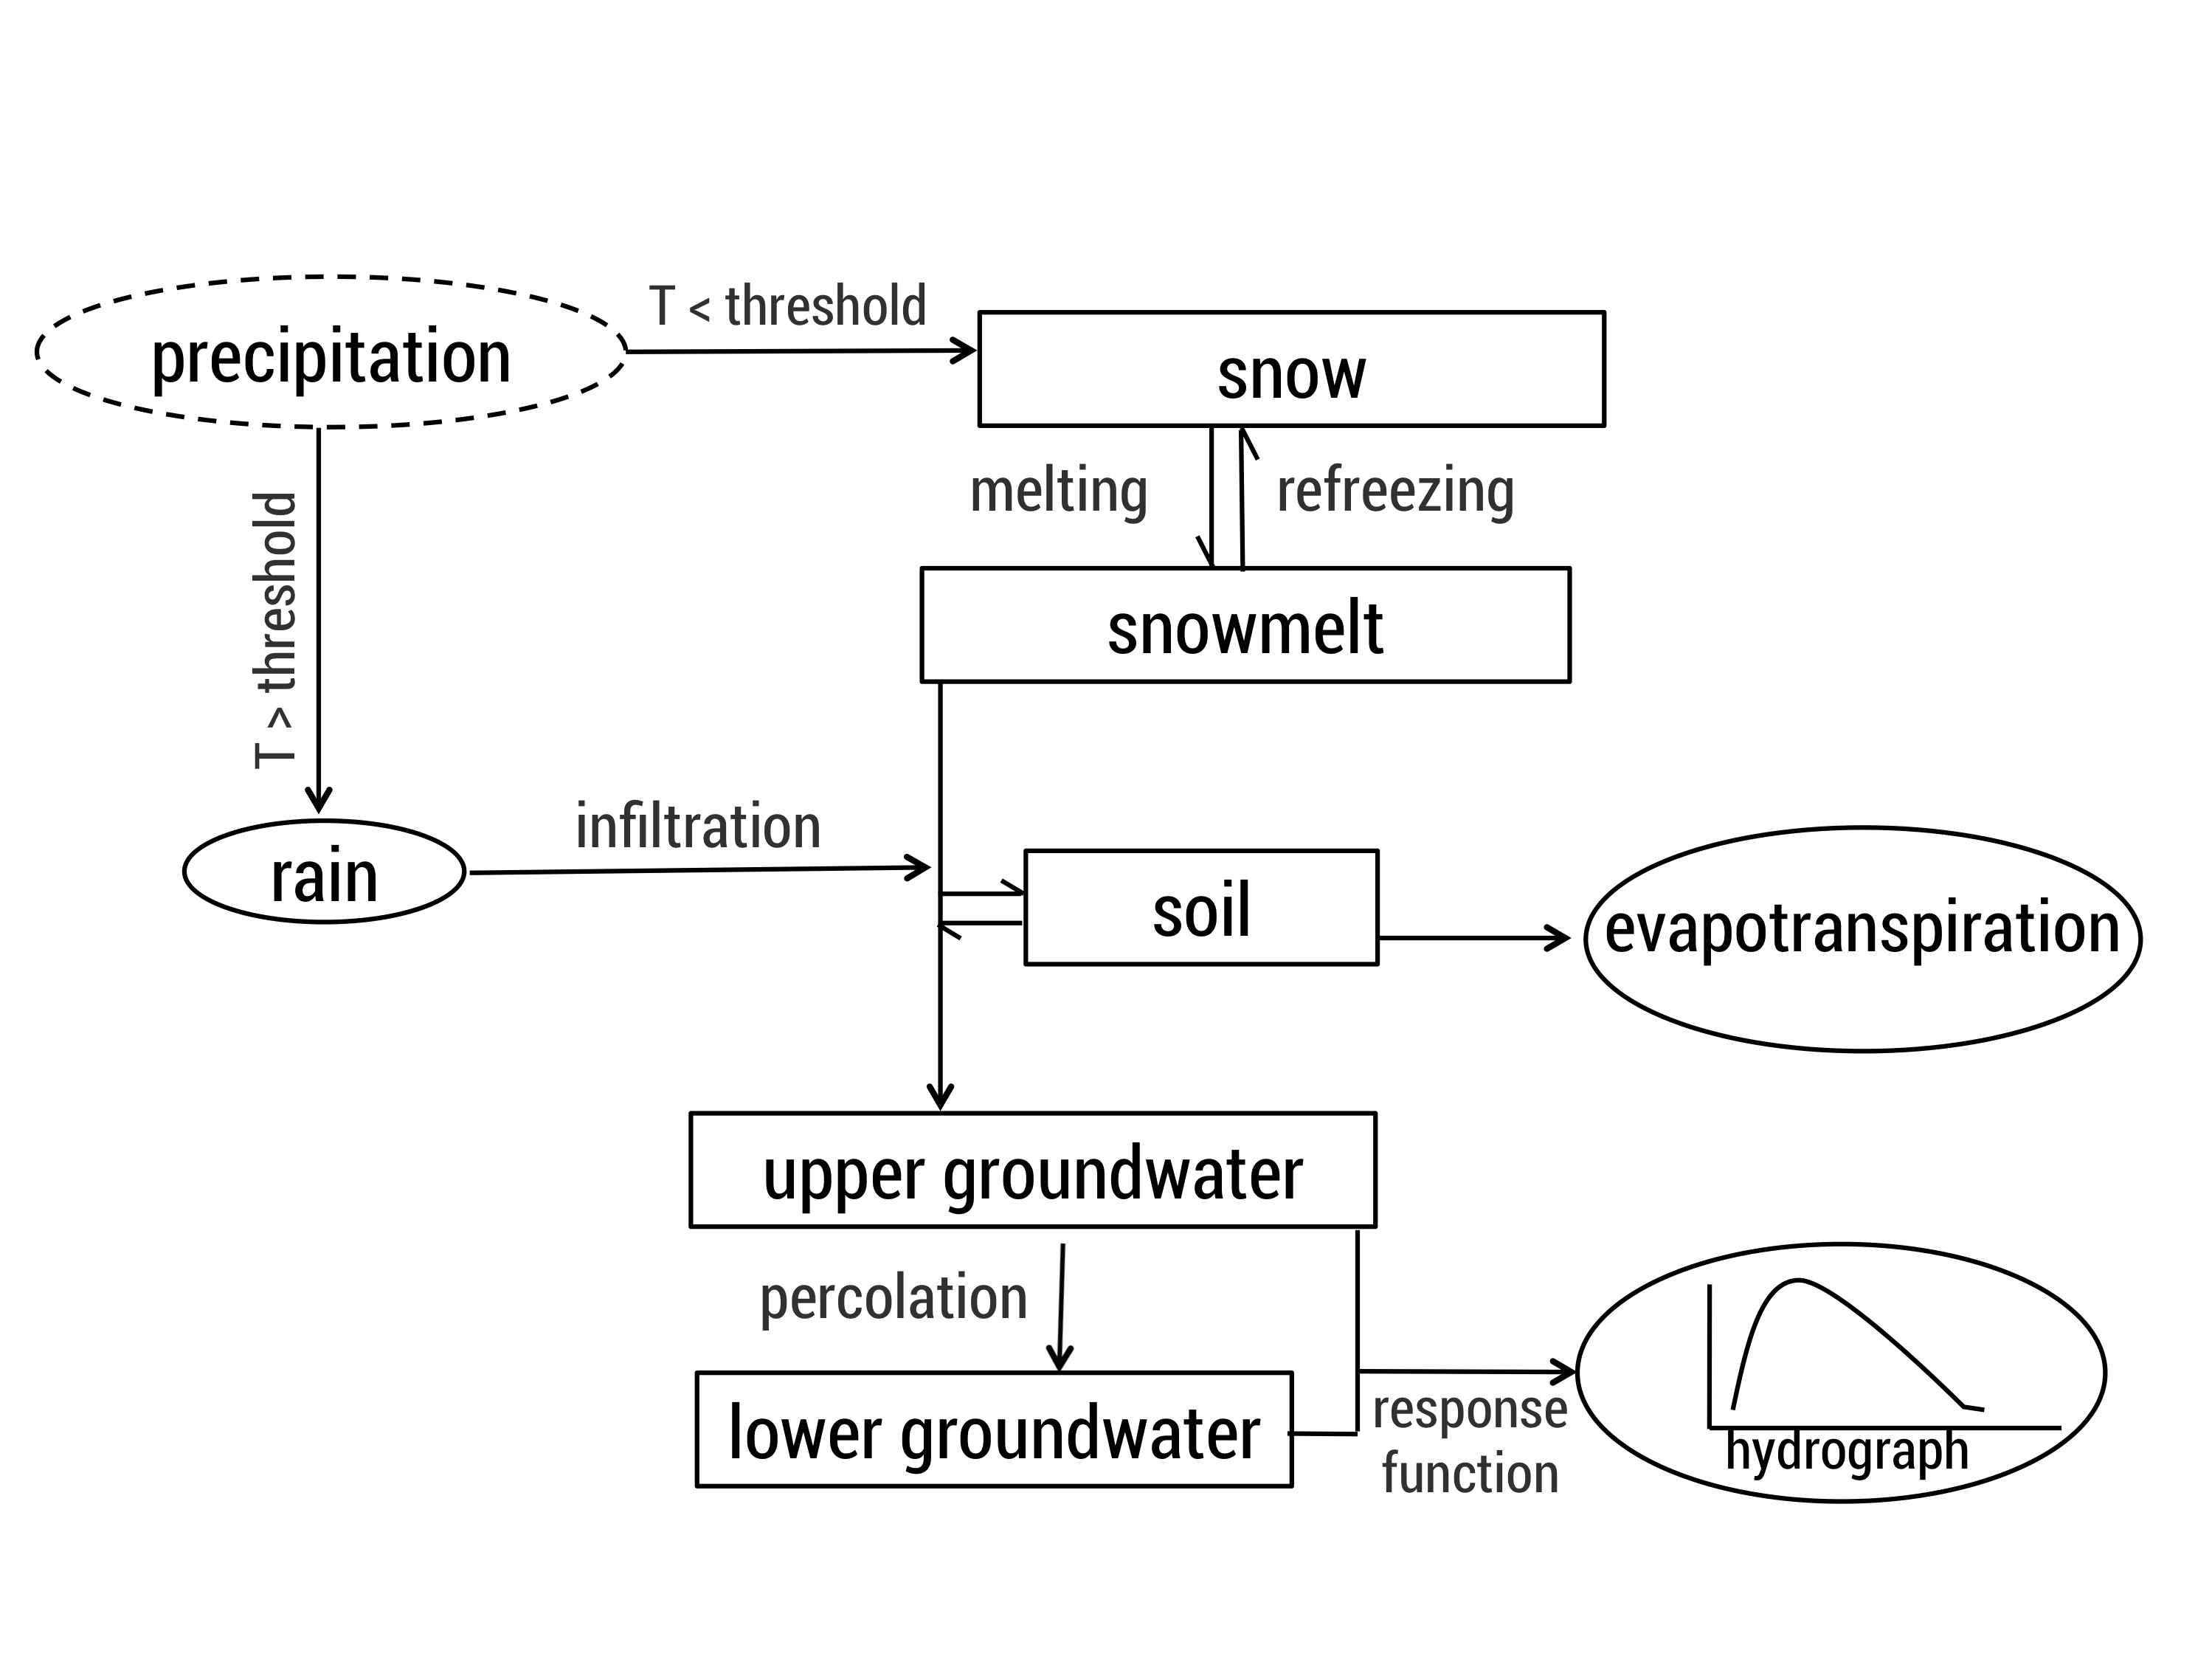
\includegraphics[width=\textwidth]{figure-files/figure3.png}
\caption{Flowchart of the different hydrologic processes and reservoirs within the Flow model in Envision, \citep[modified from][]{Han:2017tx}}
\label{fig:ModelFlowchart}
\end{figure}
\clearpage

\begin{figure}
\centering
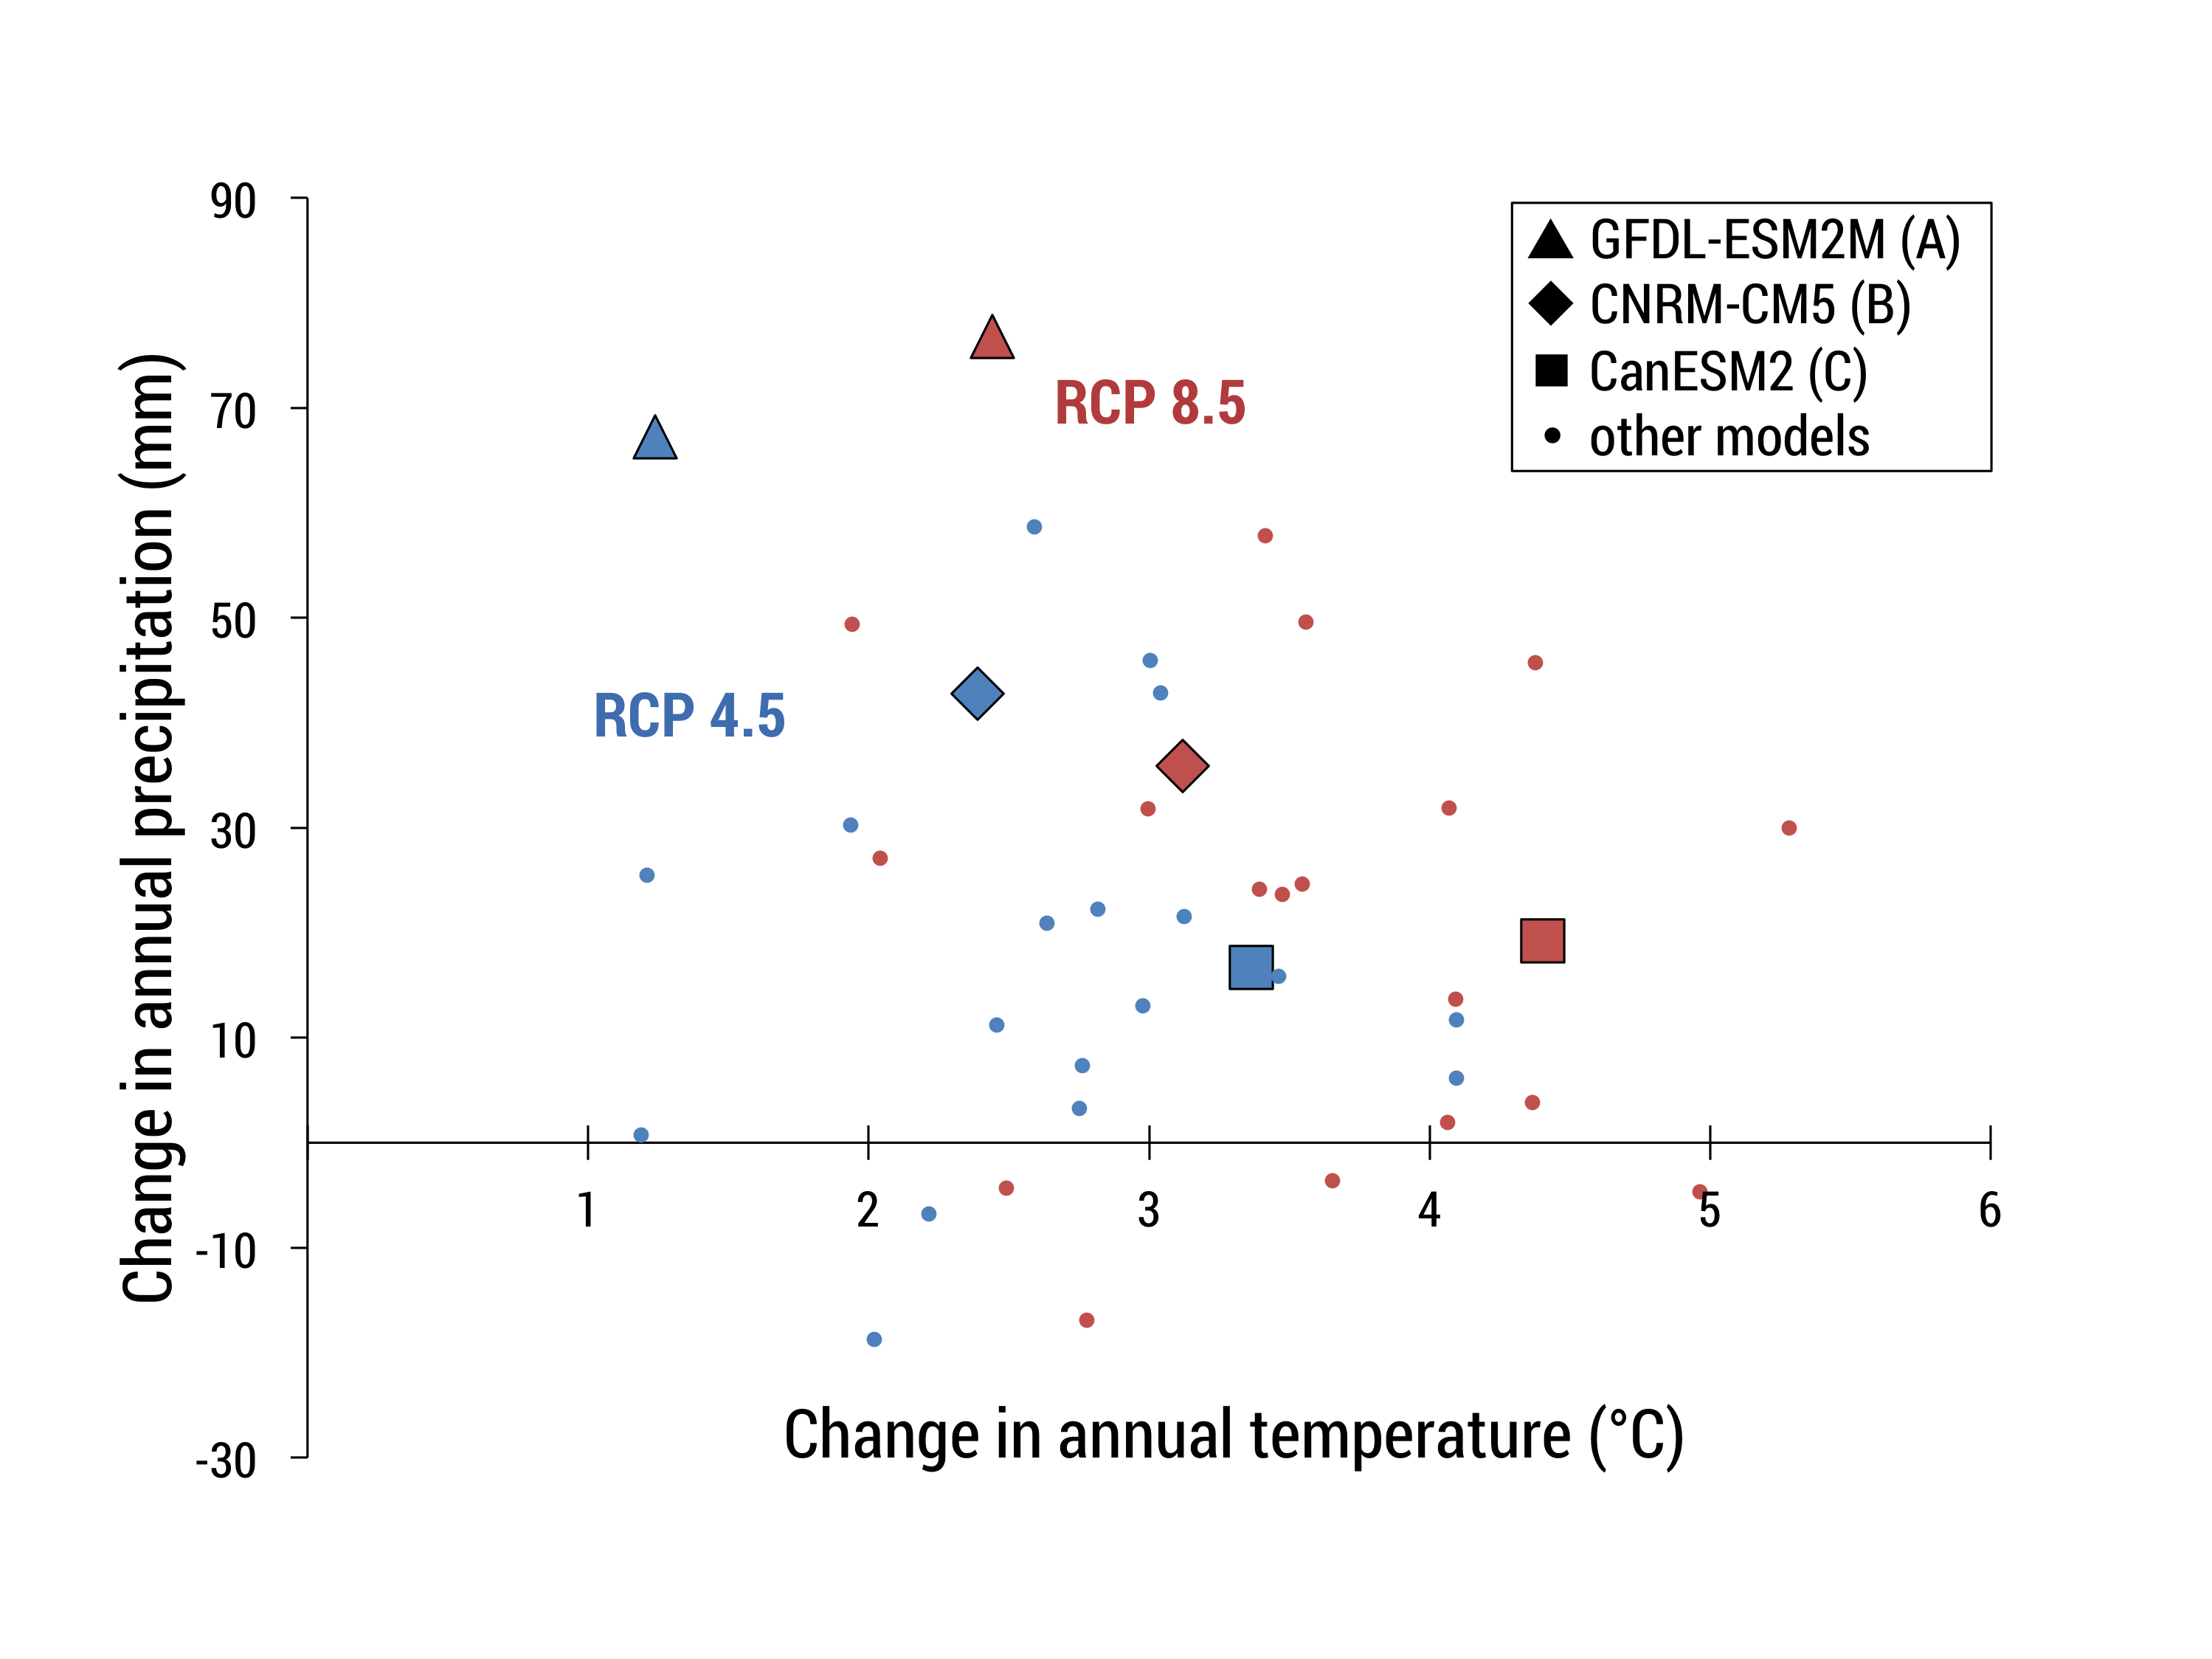
\includegraphics[width=\textwidth]{figure-files/figure4.png}
\caption{Change in climate variables from 1979-2000 to 2040-2069 for MACA downscaled GCMs \citep{Abatzoglou:2011kca}. Blue and red points represent RCP 4.5 and 8.5 scenarios, respectively. The larger icons represent the GCMs selected for this study.}
\label{fig:ClimateChange}
\end{figure}
\clearpage

\begin{figure}
\centering
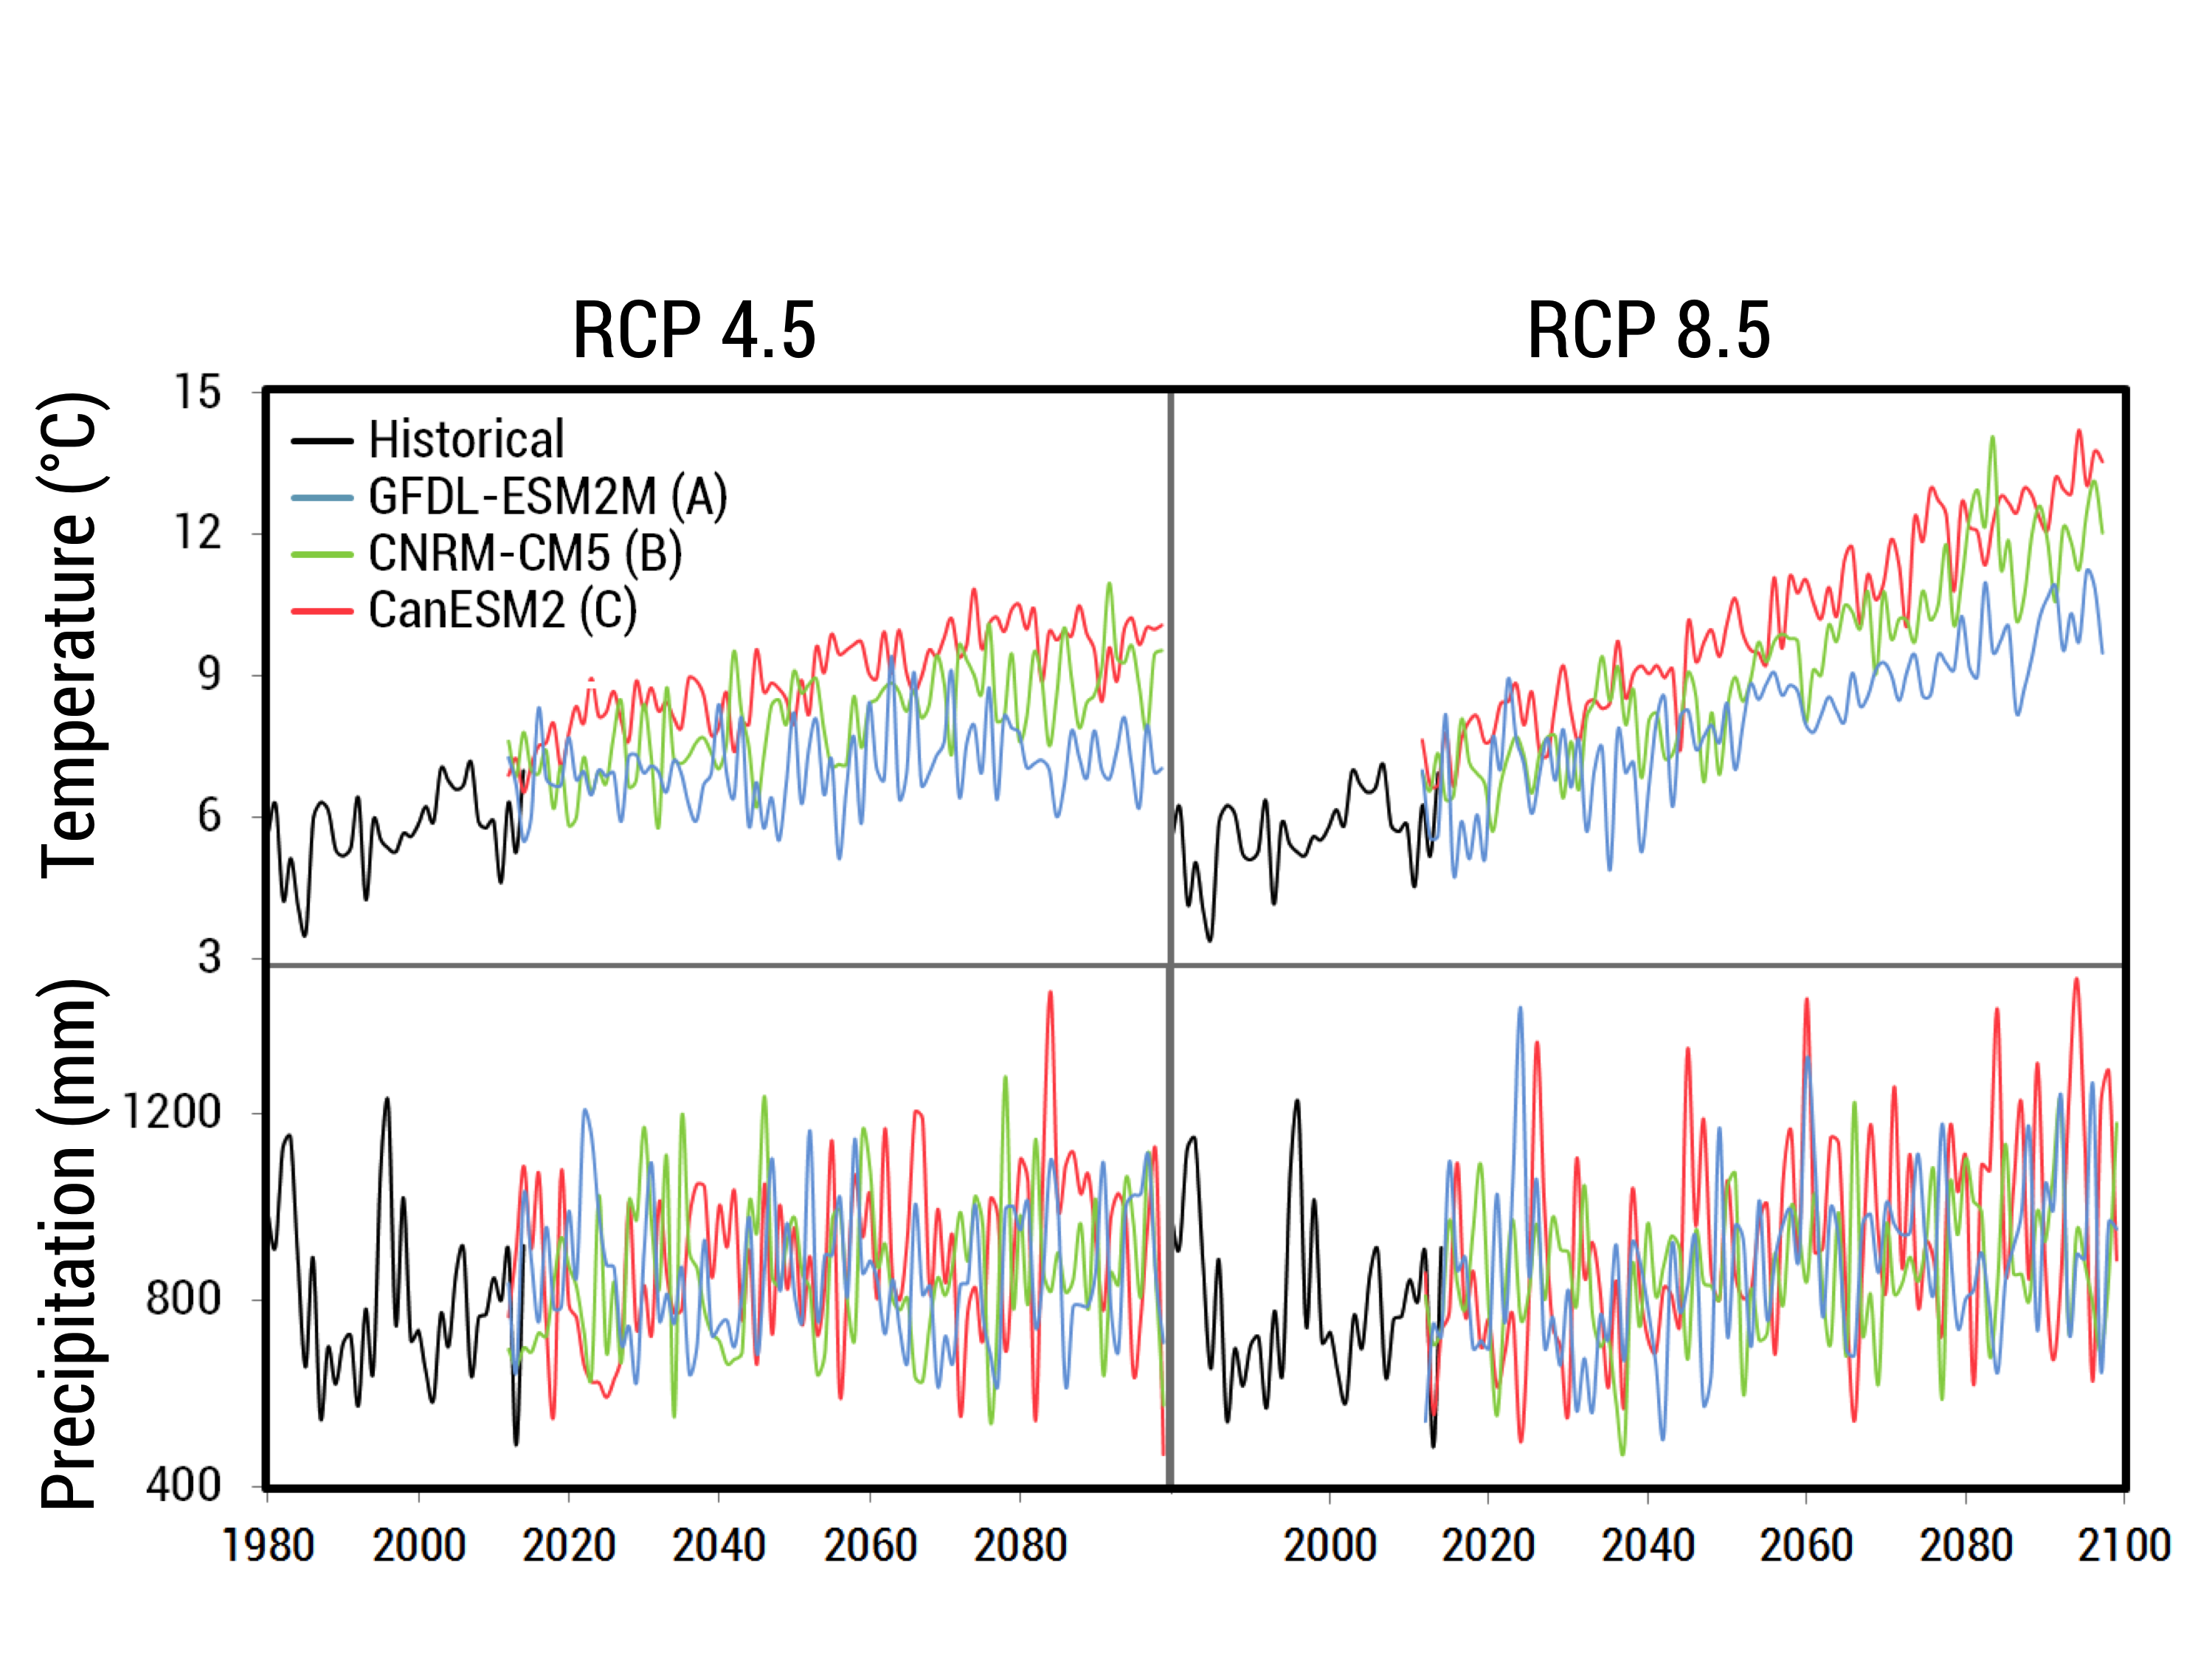
\includegraphics[width=\textwidth]{figure-files/figure5.png}
\caption{Temporal projections for annual mean temperature and precipitation for the six climate scenarios used in this study. Temperature increases in all scenarios, but precipitation is more variable.}
\label{fig:ClimateChangeSelected}
\end{figure}
\clearpage

\begin{figure}
\centering
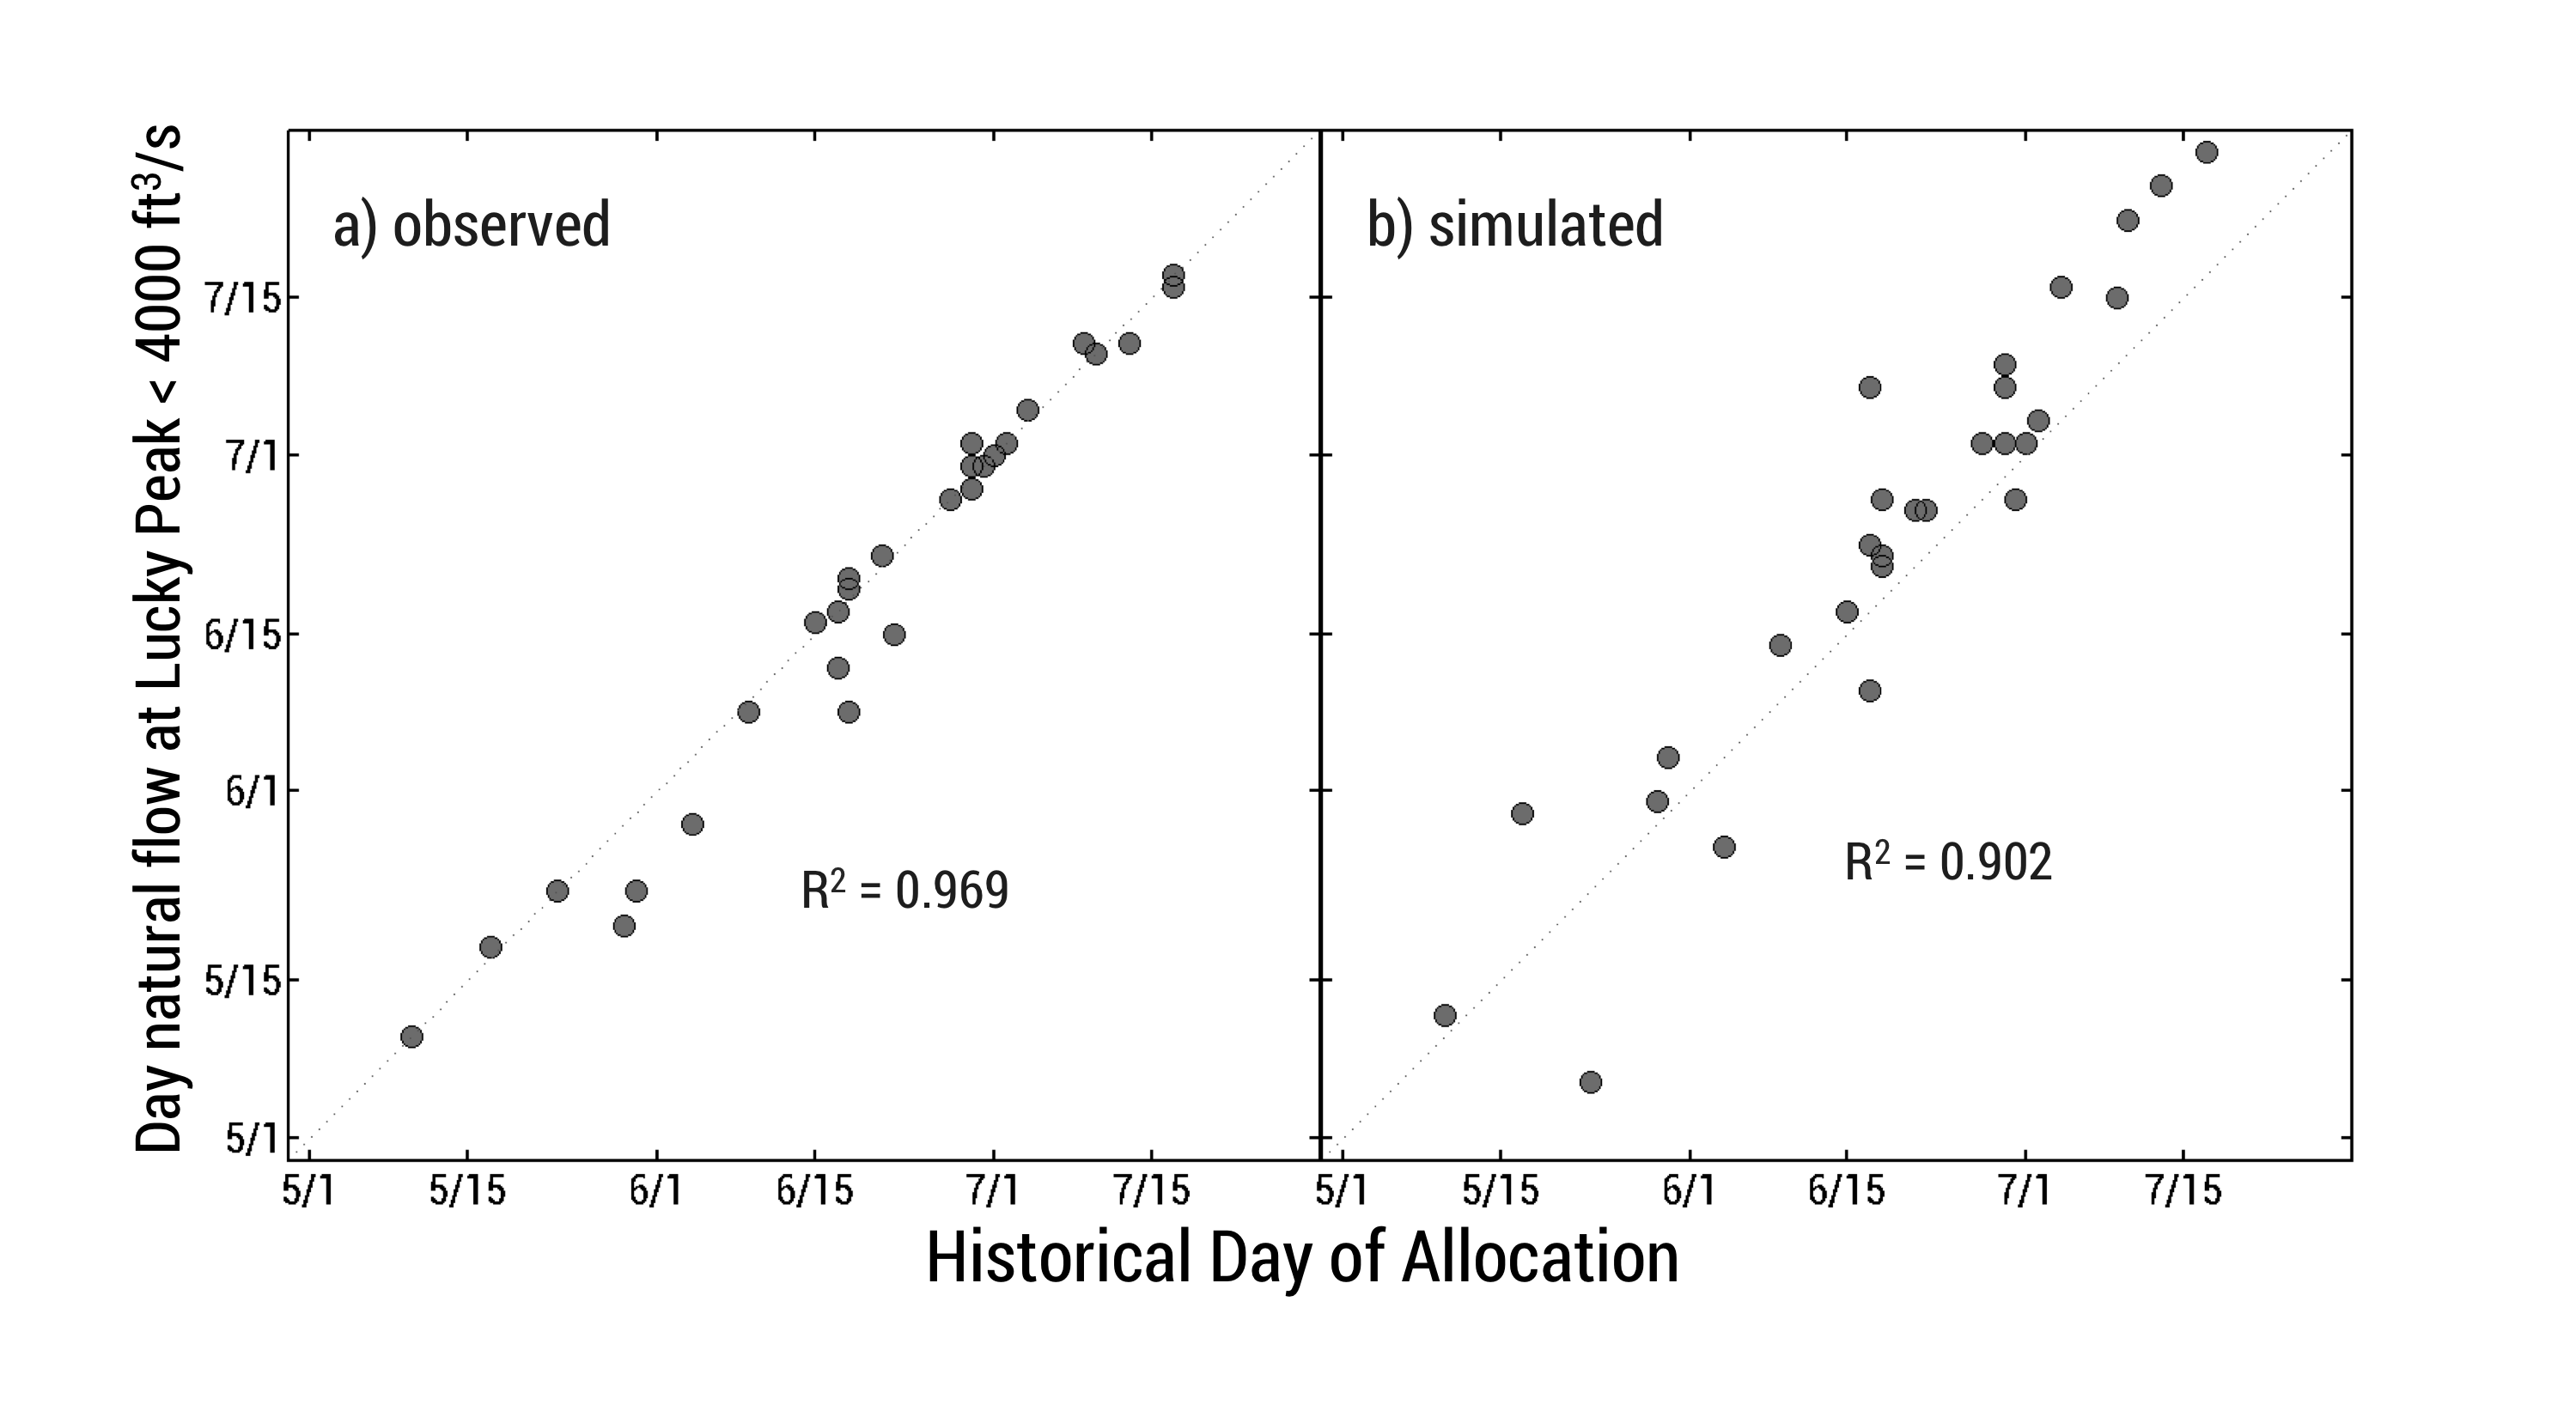
\includegraphics[width=\textwidth]{figure-files/figure6.png}
\caption{(a) Relationship between the day natural flow at Lucky Peak reaches below 4000 ft3/s and the date the Day of Allocation is declared, modified from \citep{Garst:2017bg}.  (b) Our modeled historical Day of Allocation using the same method as (a). Dashed line is 1:1 in both plots.}
\label{fig:DayOfAllocation}
\end{figure}
\clearpage

\begin{figure}
\centering
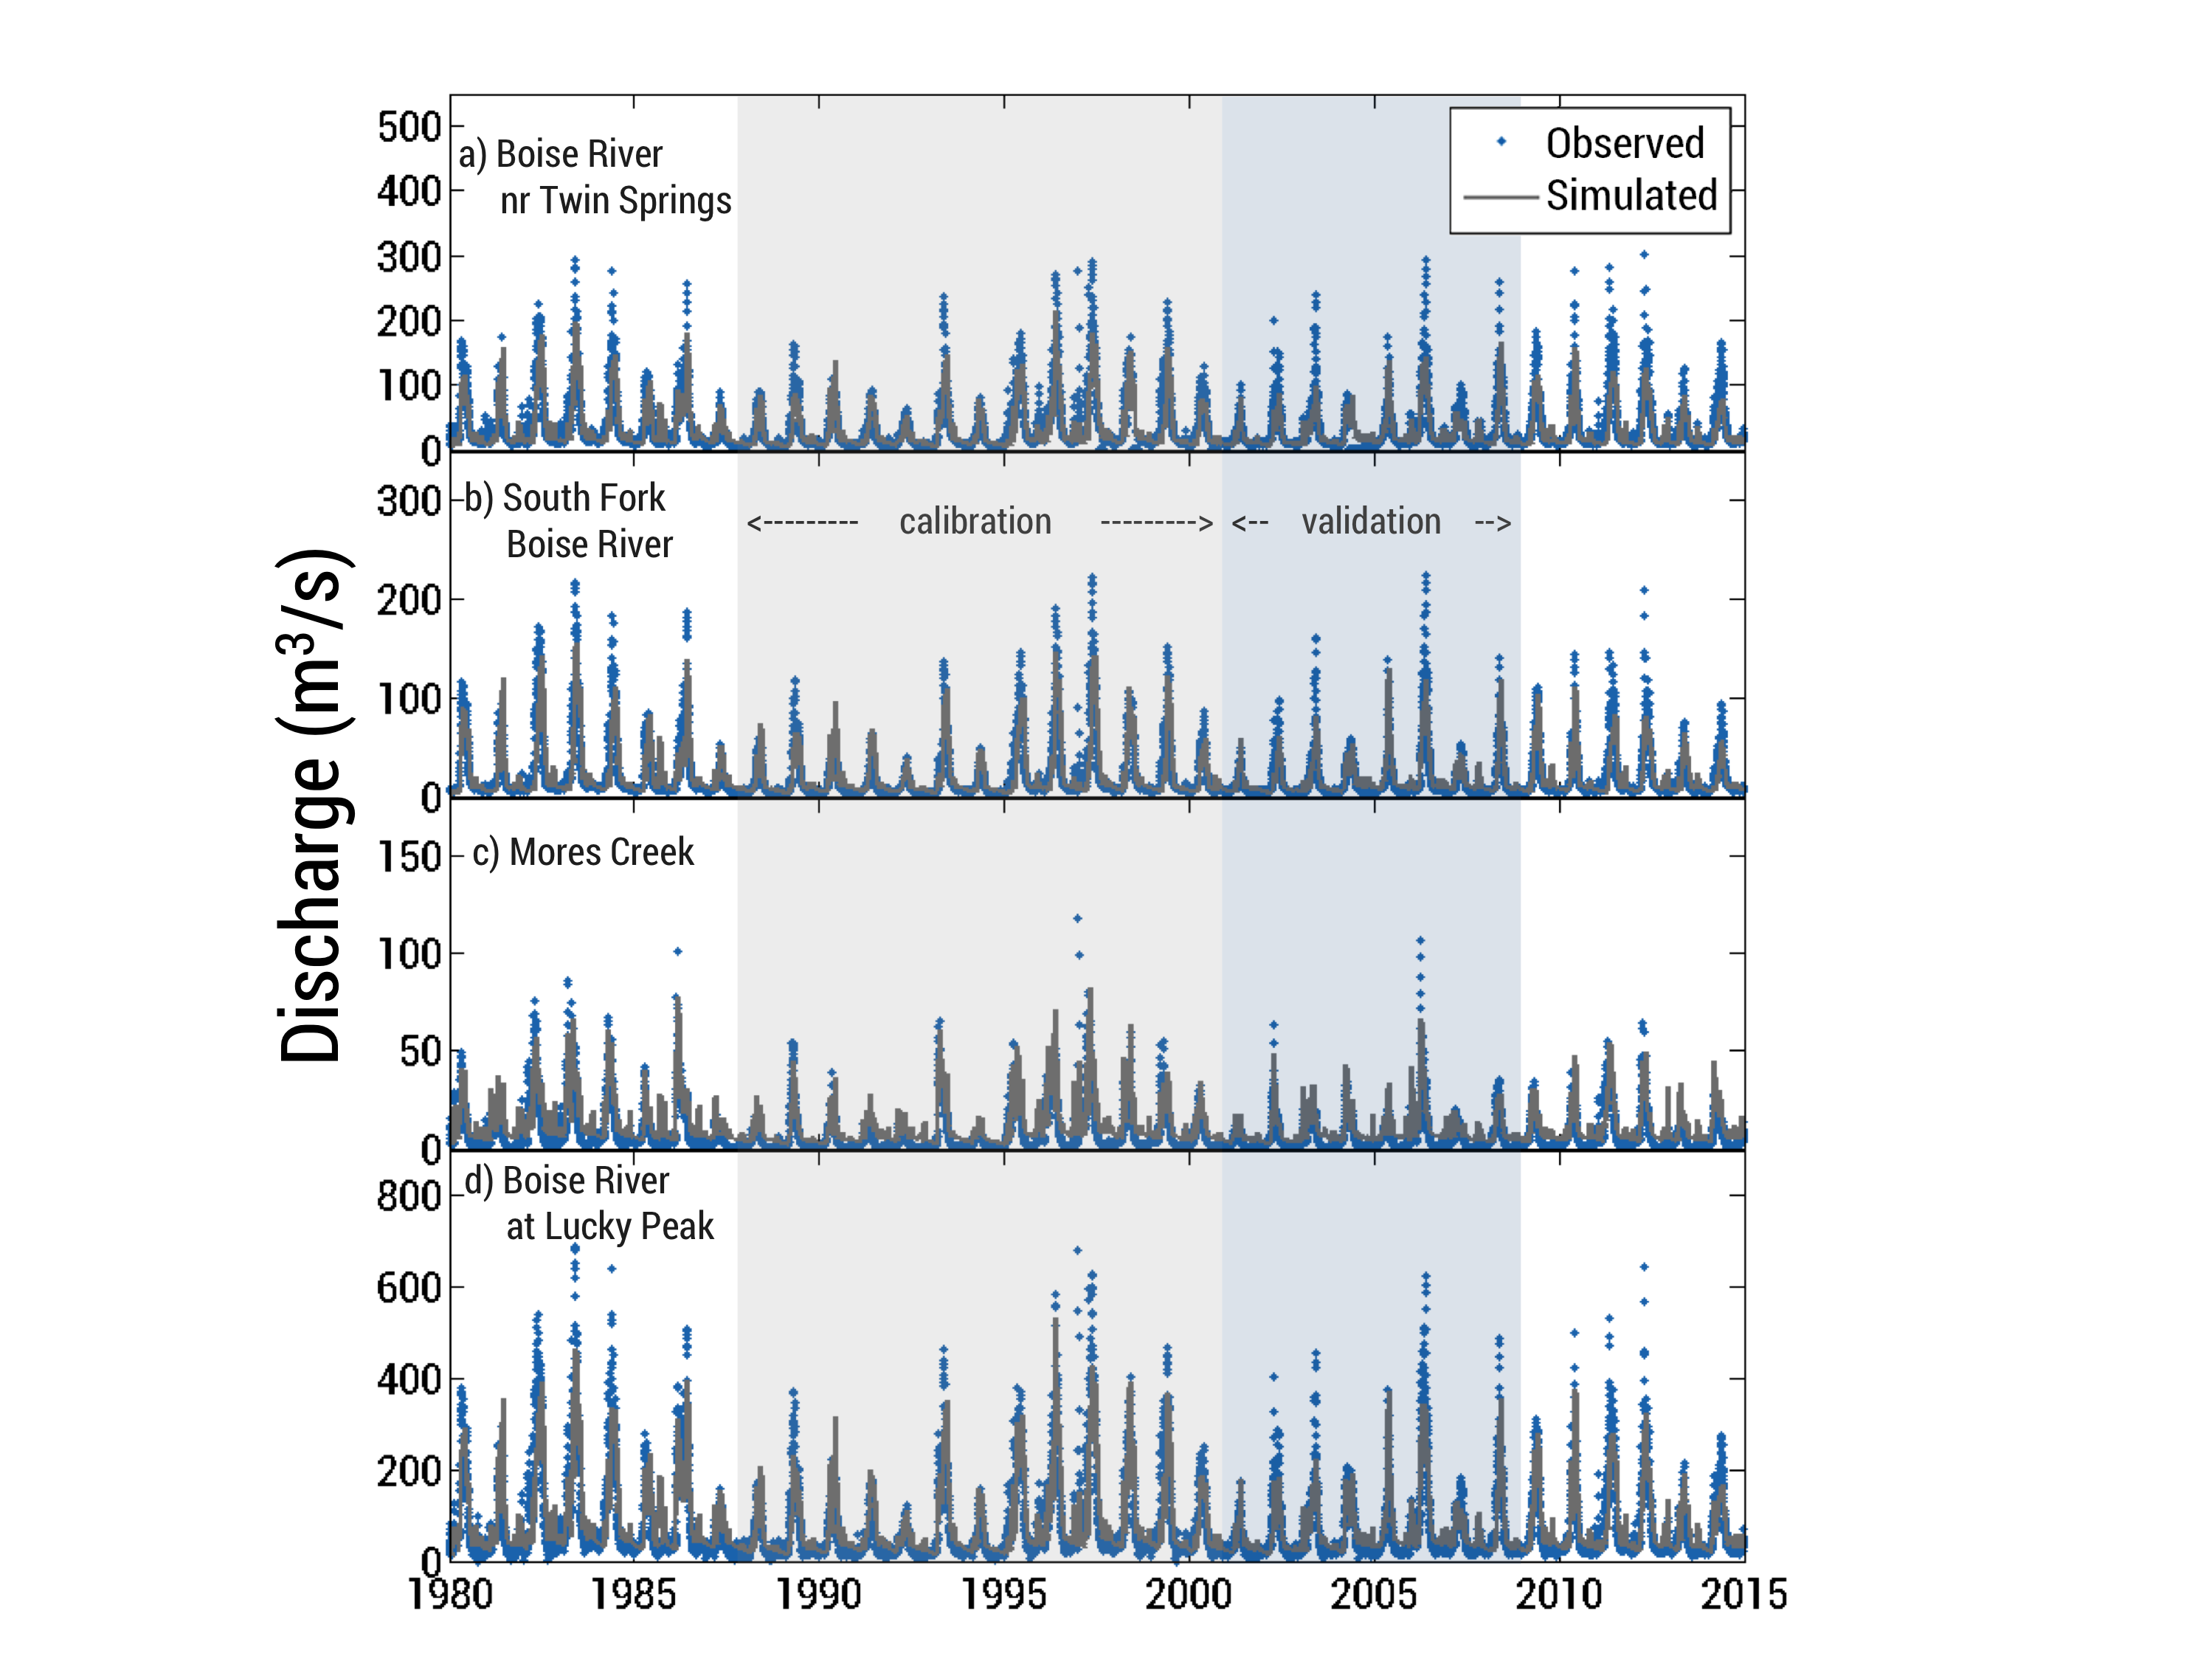
\includegraphics[width=\textwidth]{figure-files/figure7.png}
\caption{Observed and simulated streamflows during the historical period from 1980 to 2014. See Figure \ref{fig:StudySite} for locations of sites. The model does a good job at simulating historical flows, but under estimates magnitude of peak flows and over estimates baseflow at Mores Creek.}
\label{fig:CalVal}
\end{figure}
\clearpage

\begin{figure}
\centering
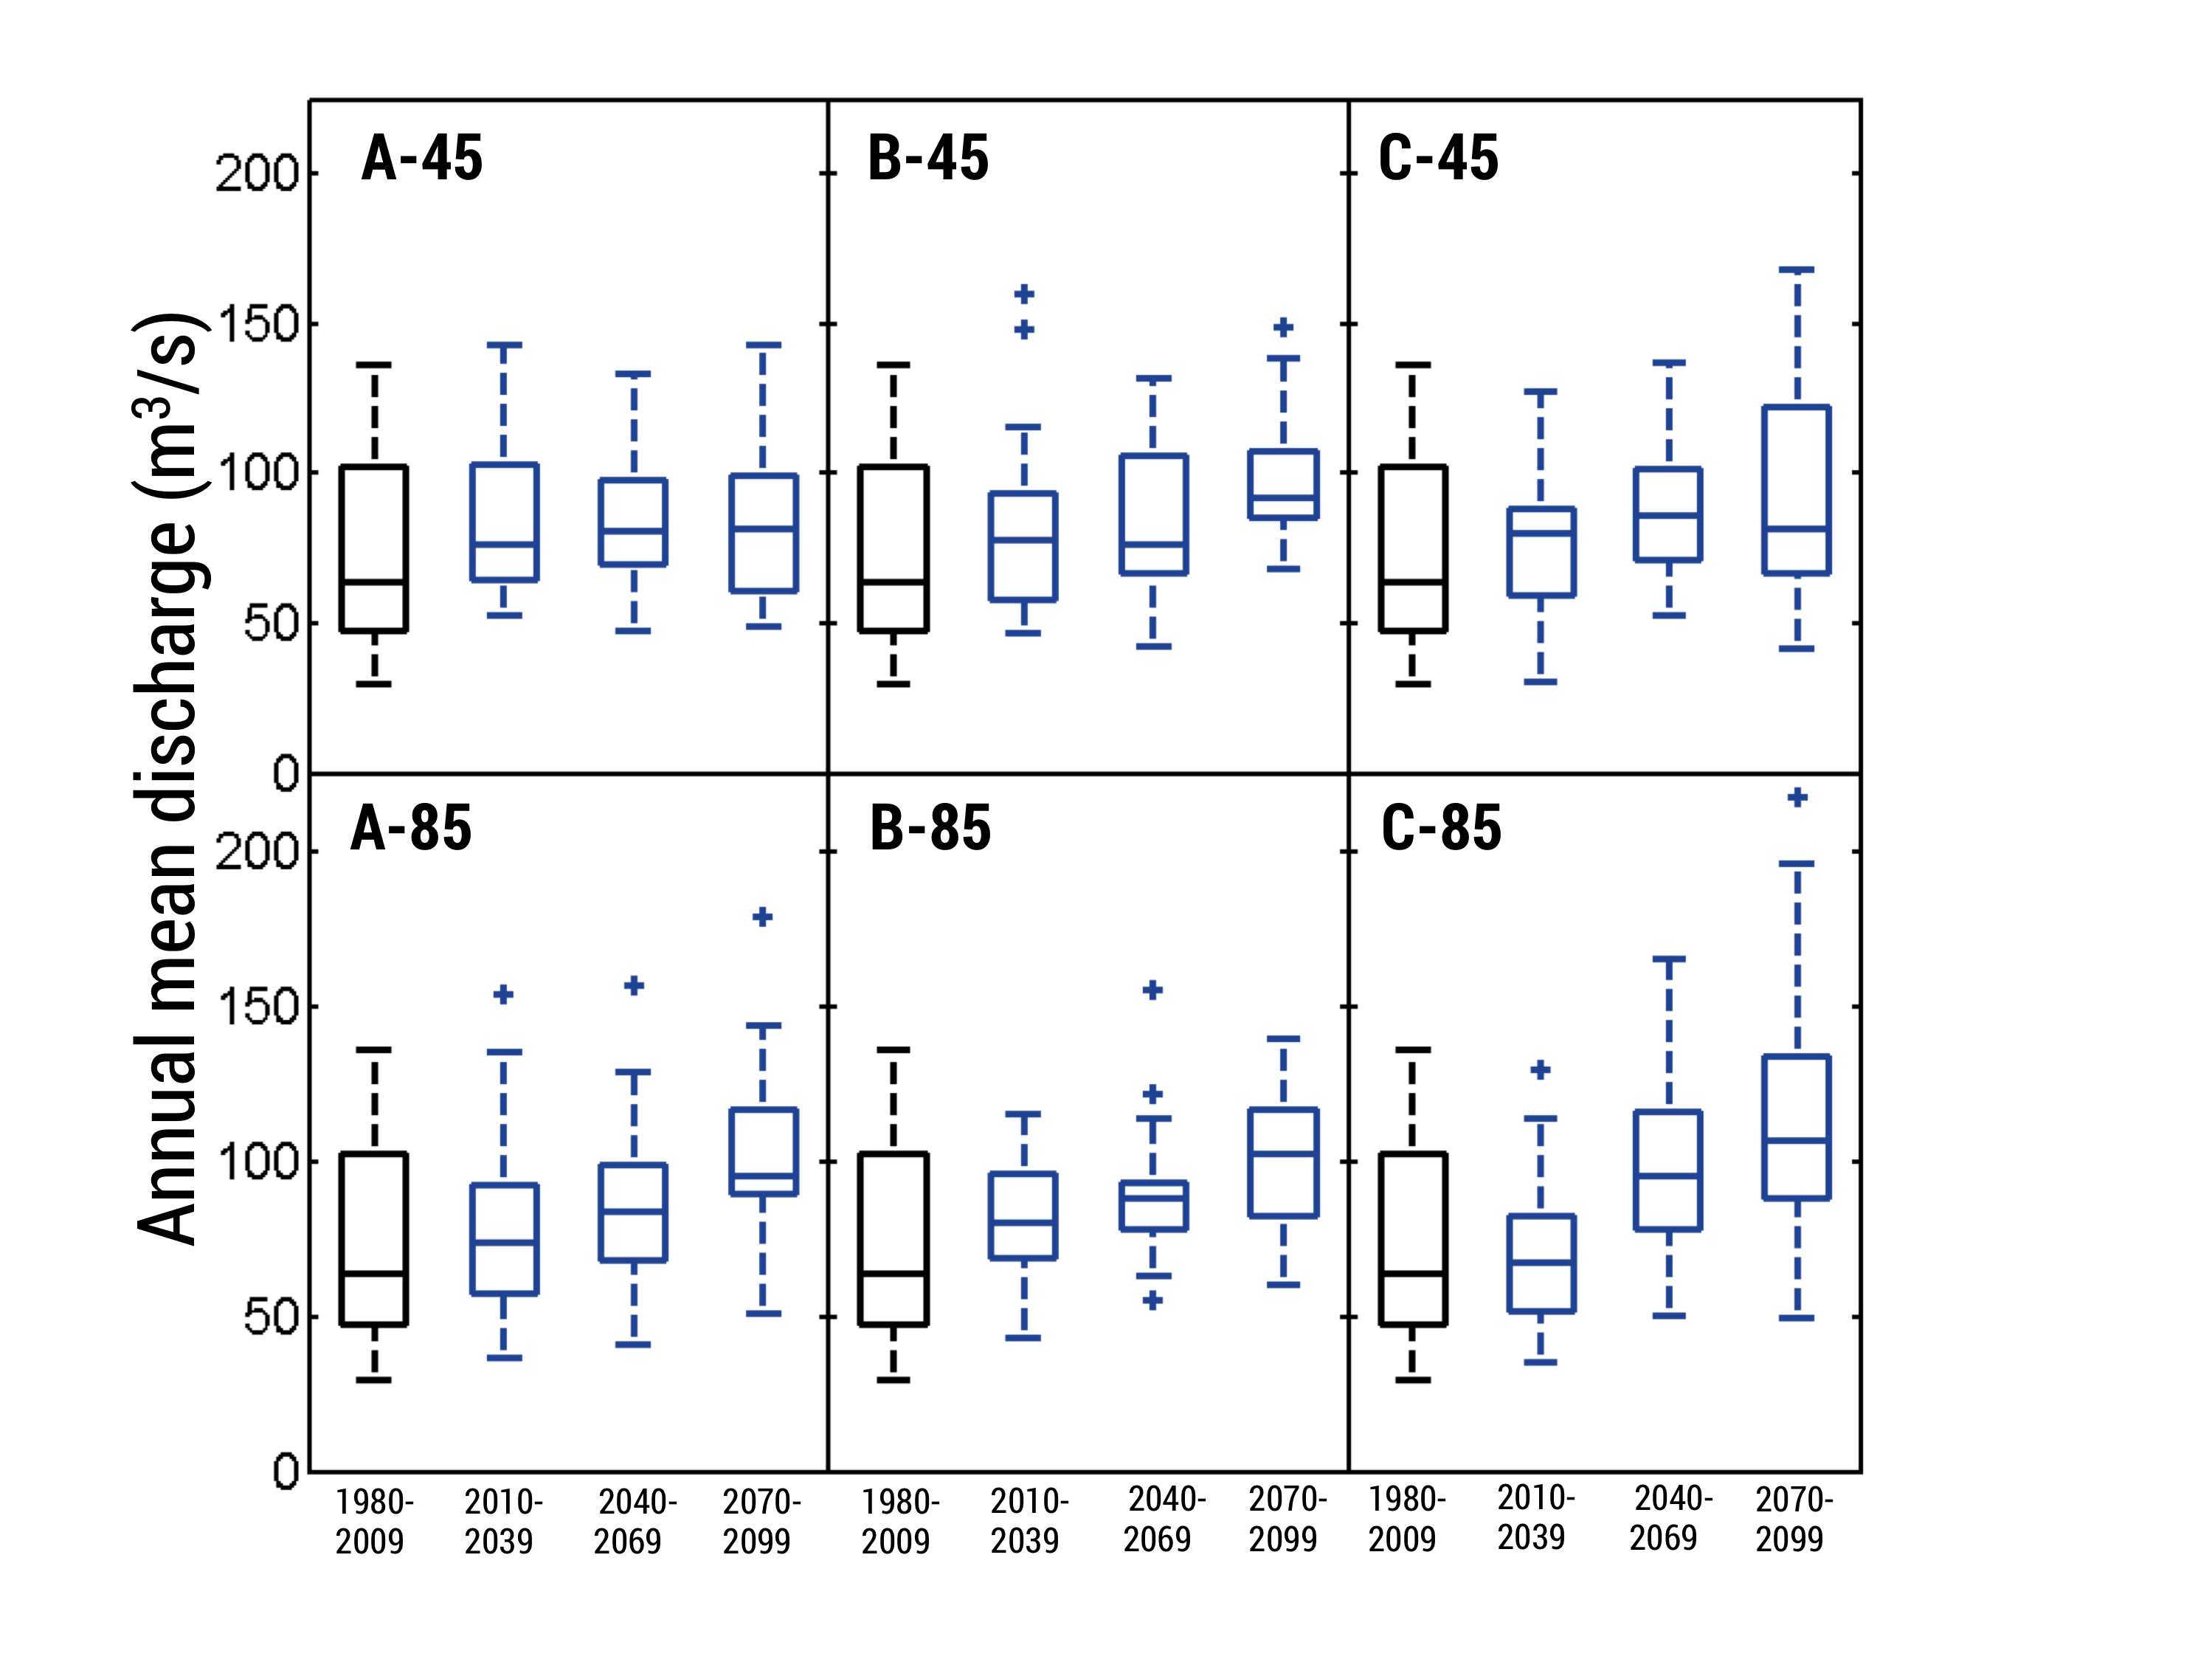
\includegraphics[width=\textwidth]{figure-files/figure8.png}
\caption{Average annual discharge of the UBRB. Values for 1980-2009 are observed. In most scenarios, we see an increase in overall discharge throughout the century. Boxes represent upper and lower quartiles and lines inside are the median.}
\label{fig:BoxPlotDischarge}
\end{figure}
\clearpage

\begin{figure}
\centering
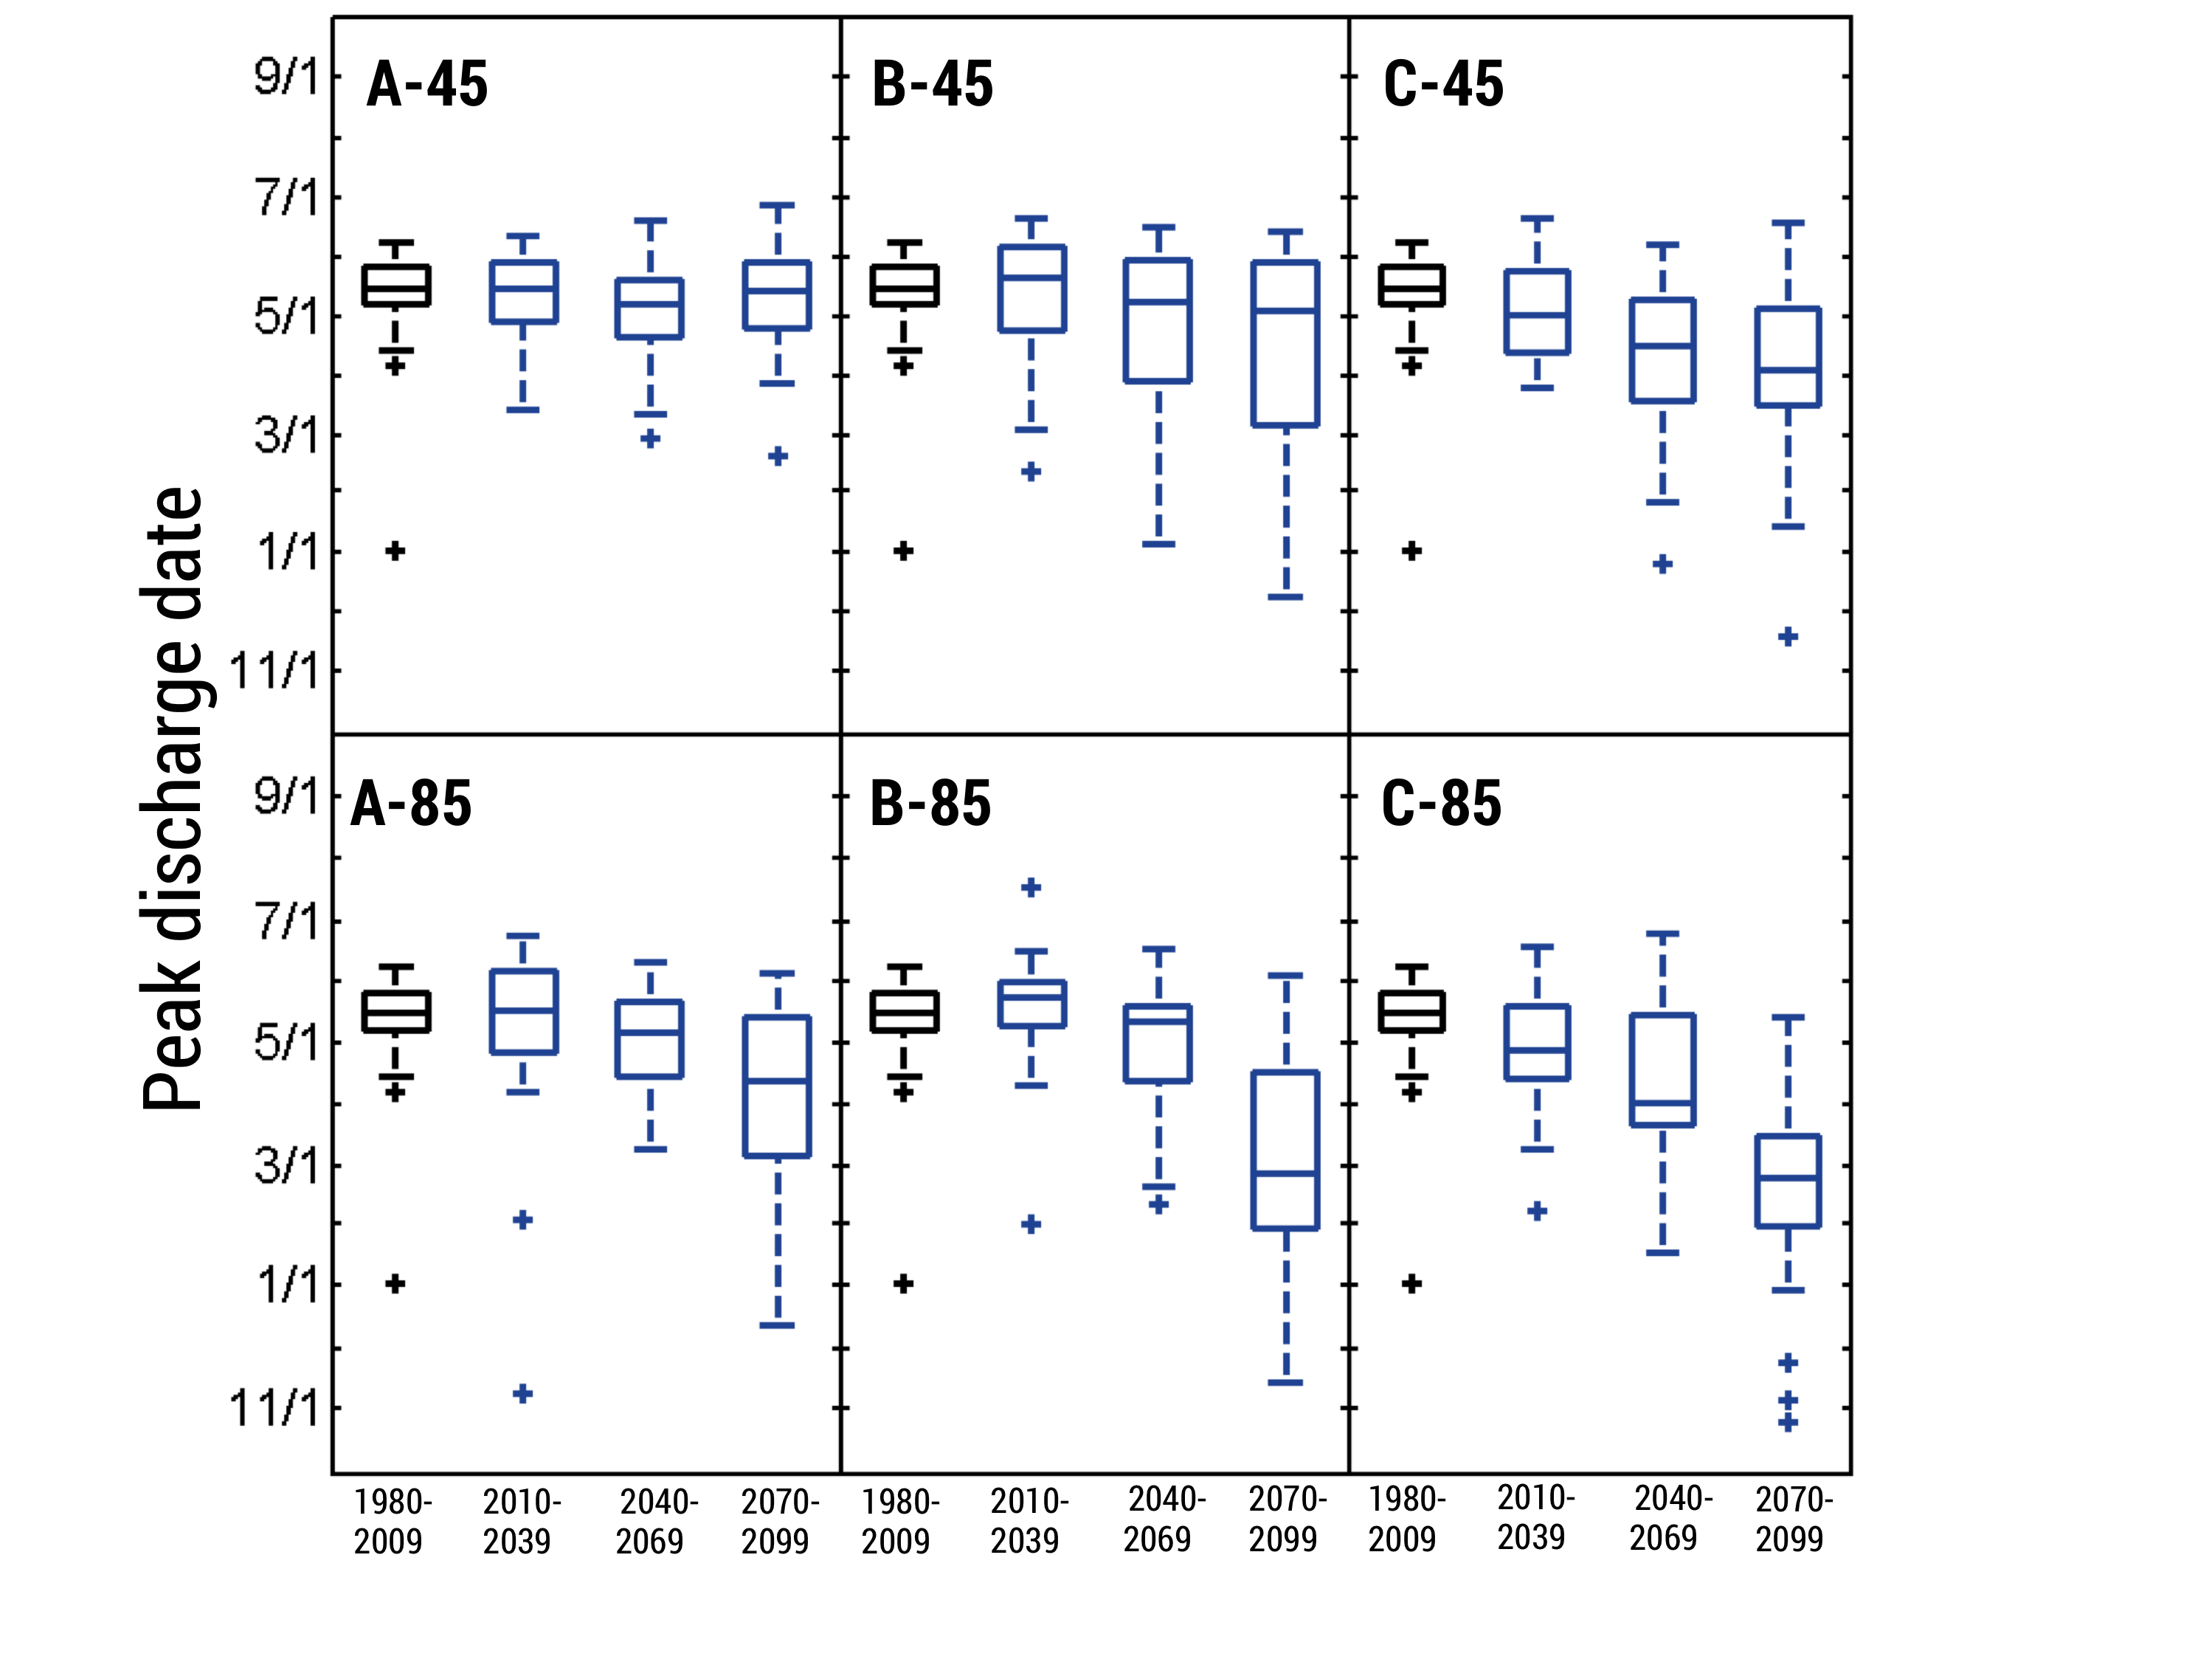
\includegraphics[width=\textwidth]{figure-files/figure9.png}
\caption{Date when peak discharge occurs for the Boise River at Lucky Peak. Values for 1980-2009 are observed. Overall, we see peak discharge date moving substantially earlier in five scenarios.}
\label{fig:PeakDischargeDate}
\end{figure}
\clearpage

\begin{figure}
\centering
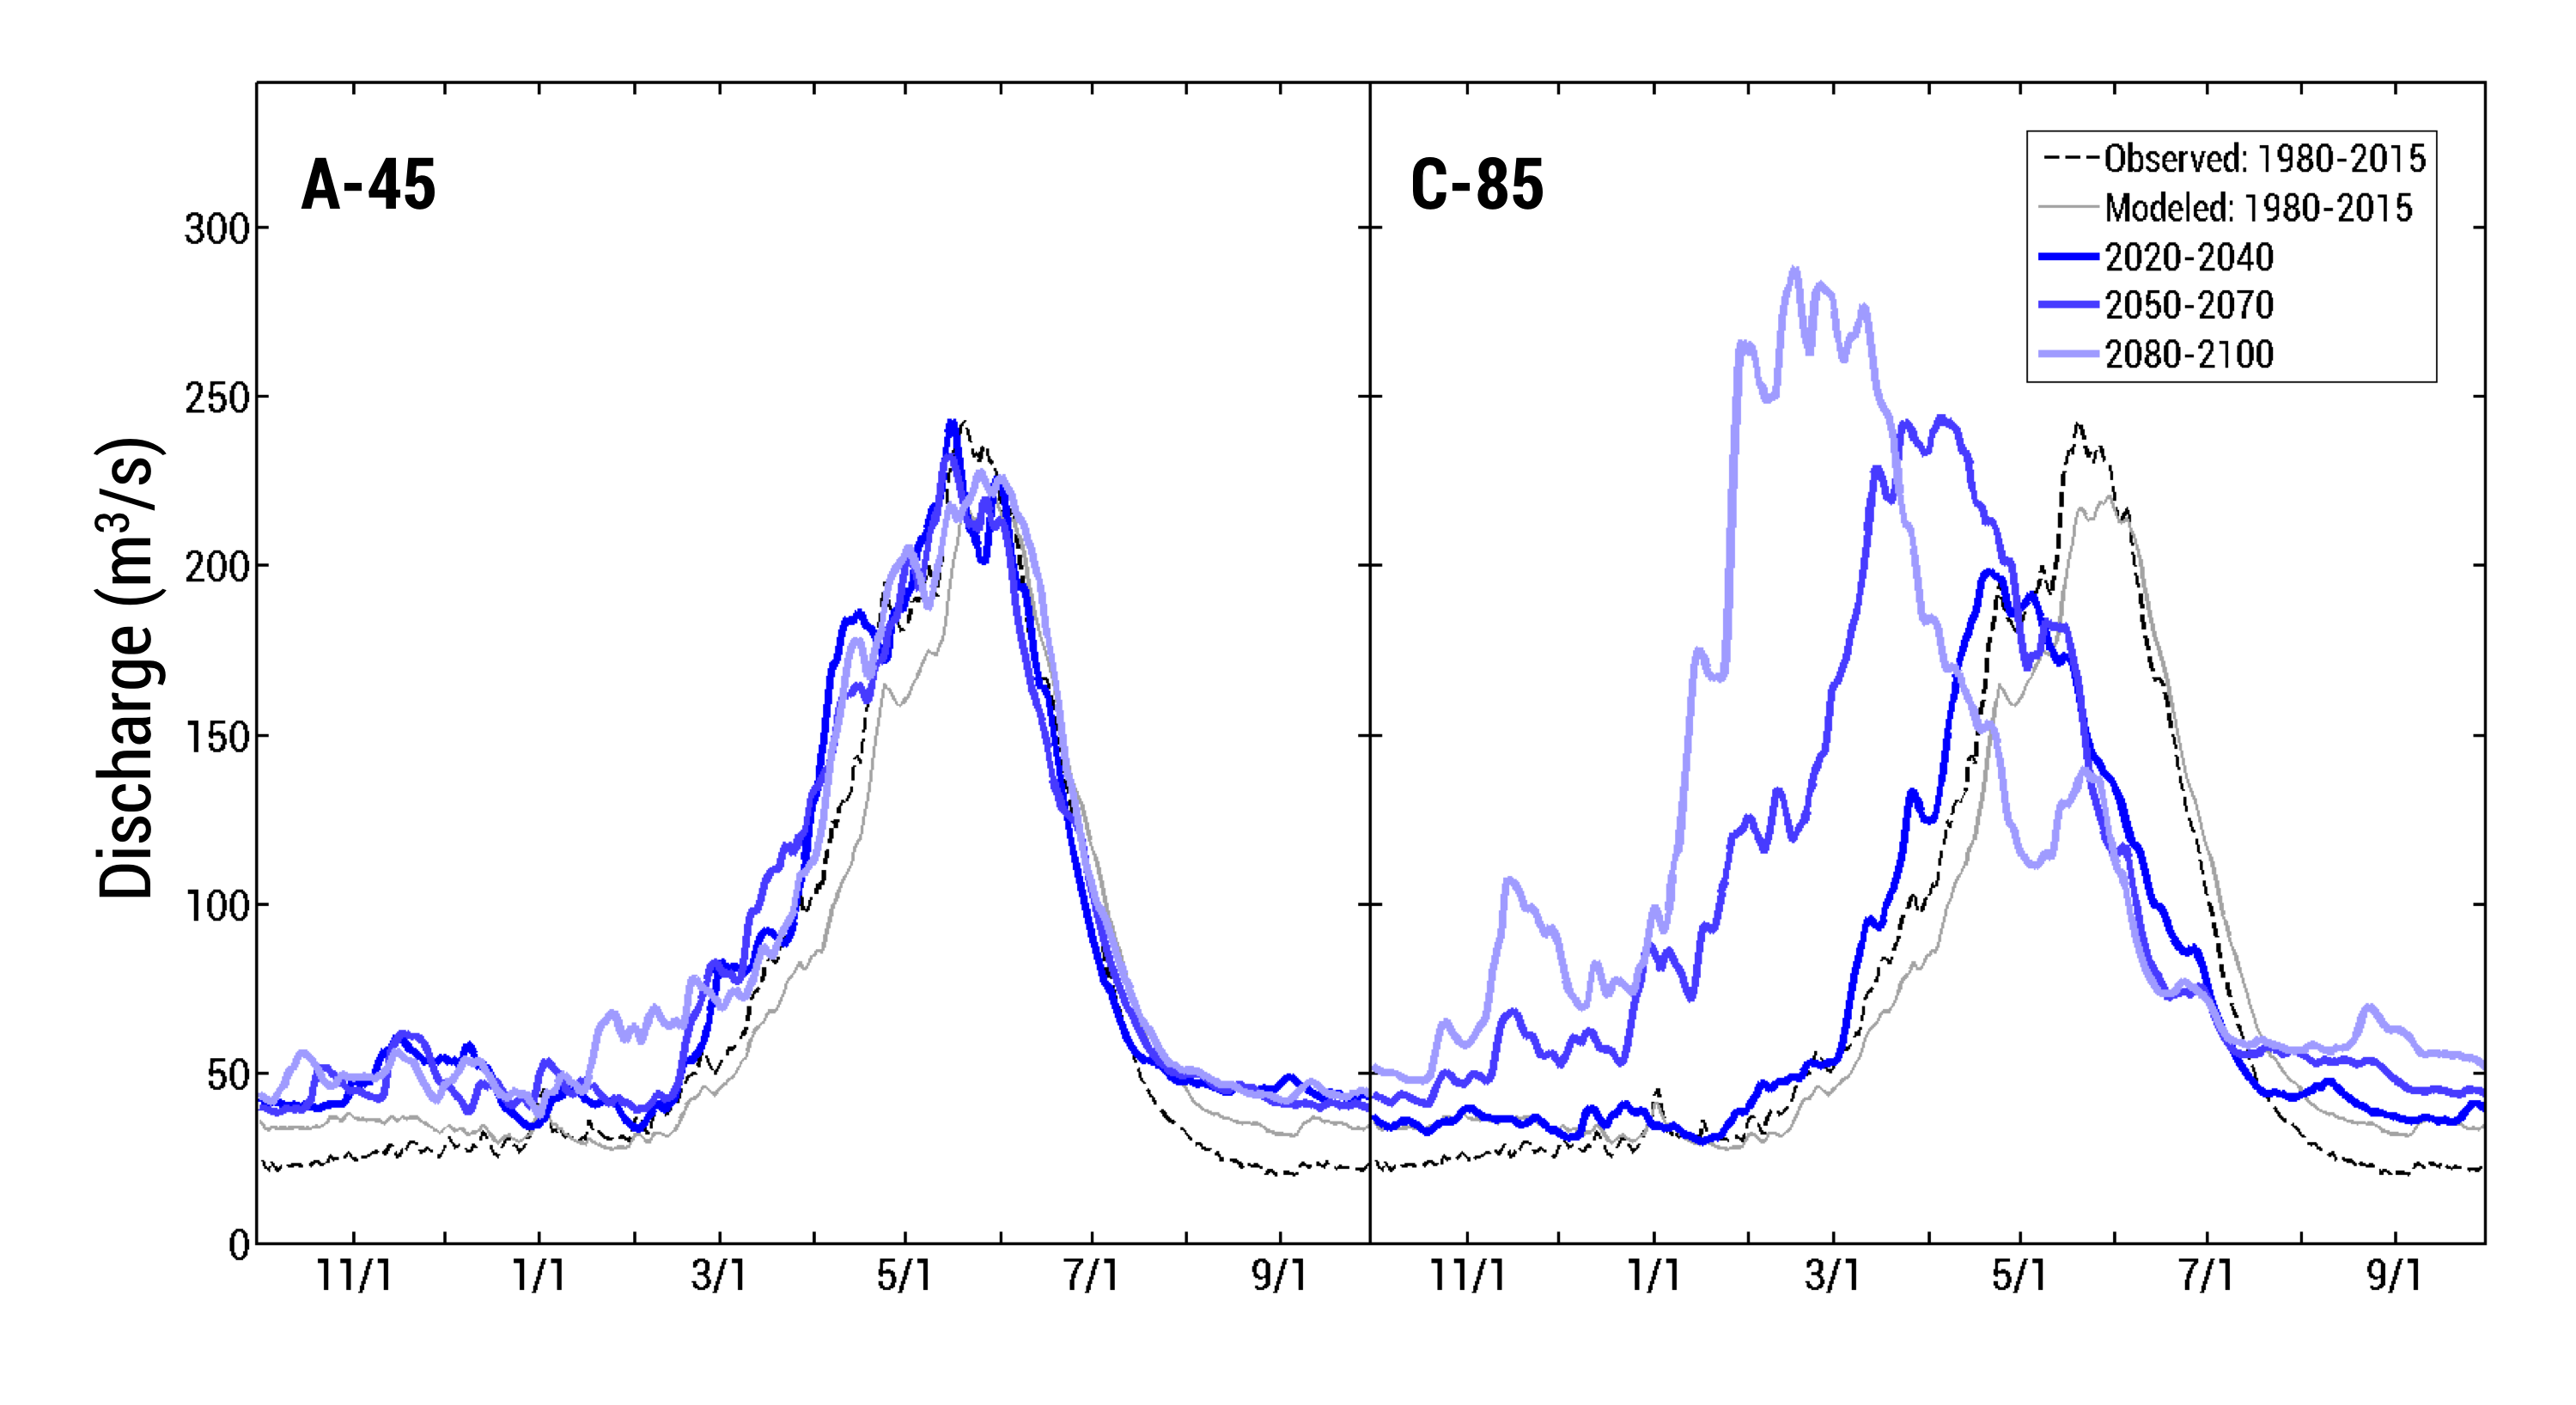
\includegraphics[width=\textwidth]{figure-files/figure10.png}
\caption{Hydrographs averaged over 2-decadal timespans for scenarios predicting the least amount of change (A-45) and the greatest amount of change (C-85) from historical.}
\label{fig:HydrographDecadeAvg}
\end{figure}
\clearpage

\begin{figure}
\centering
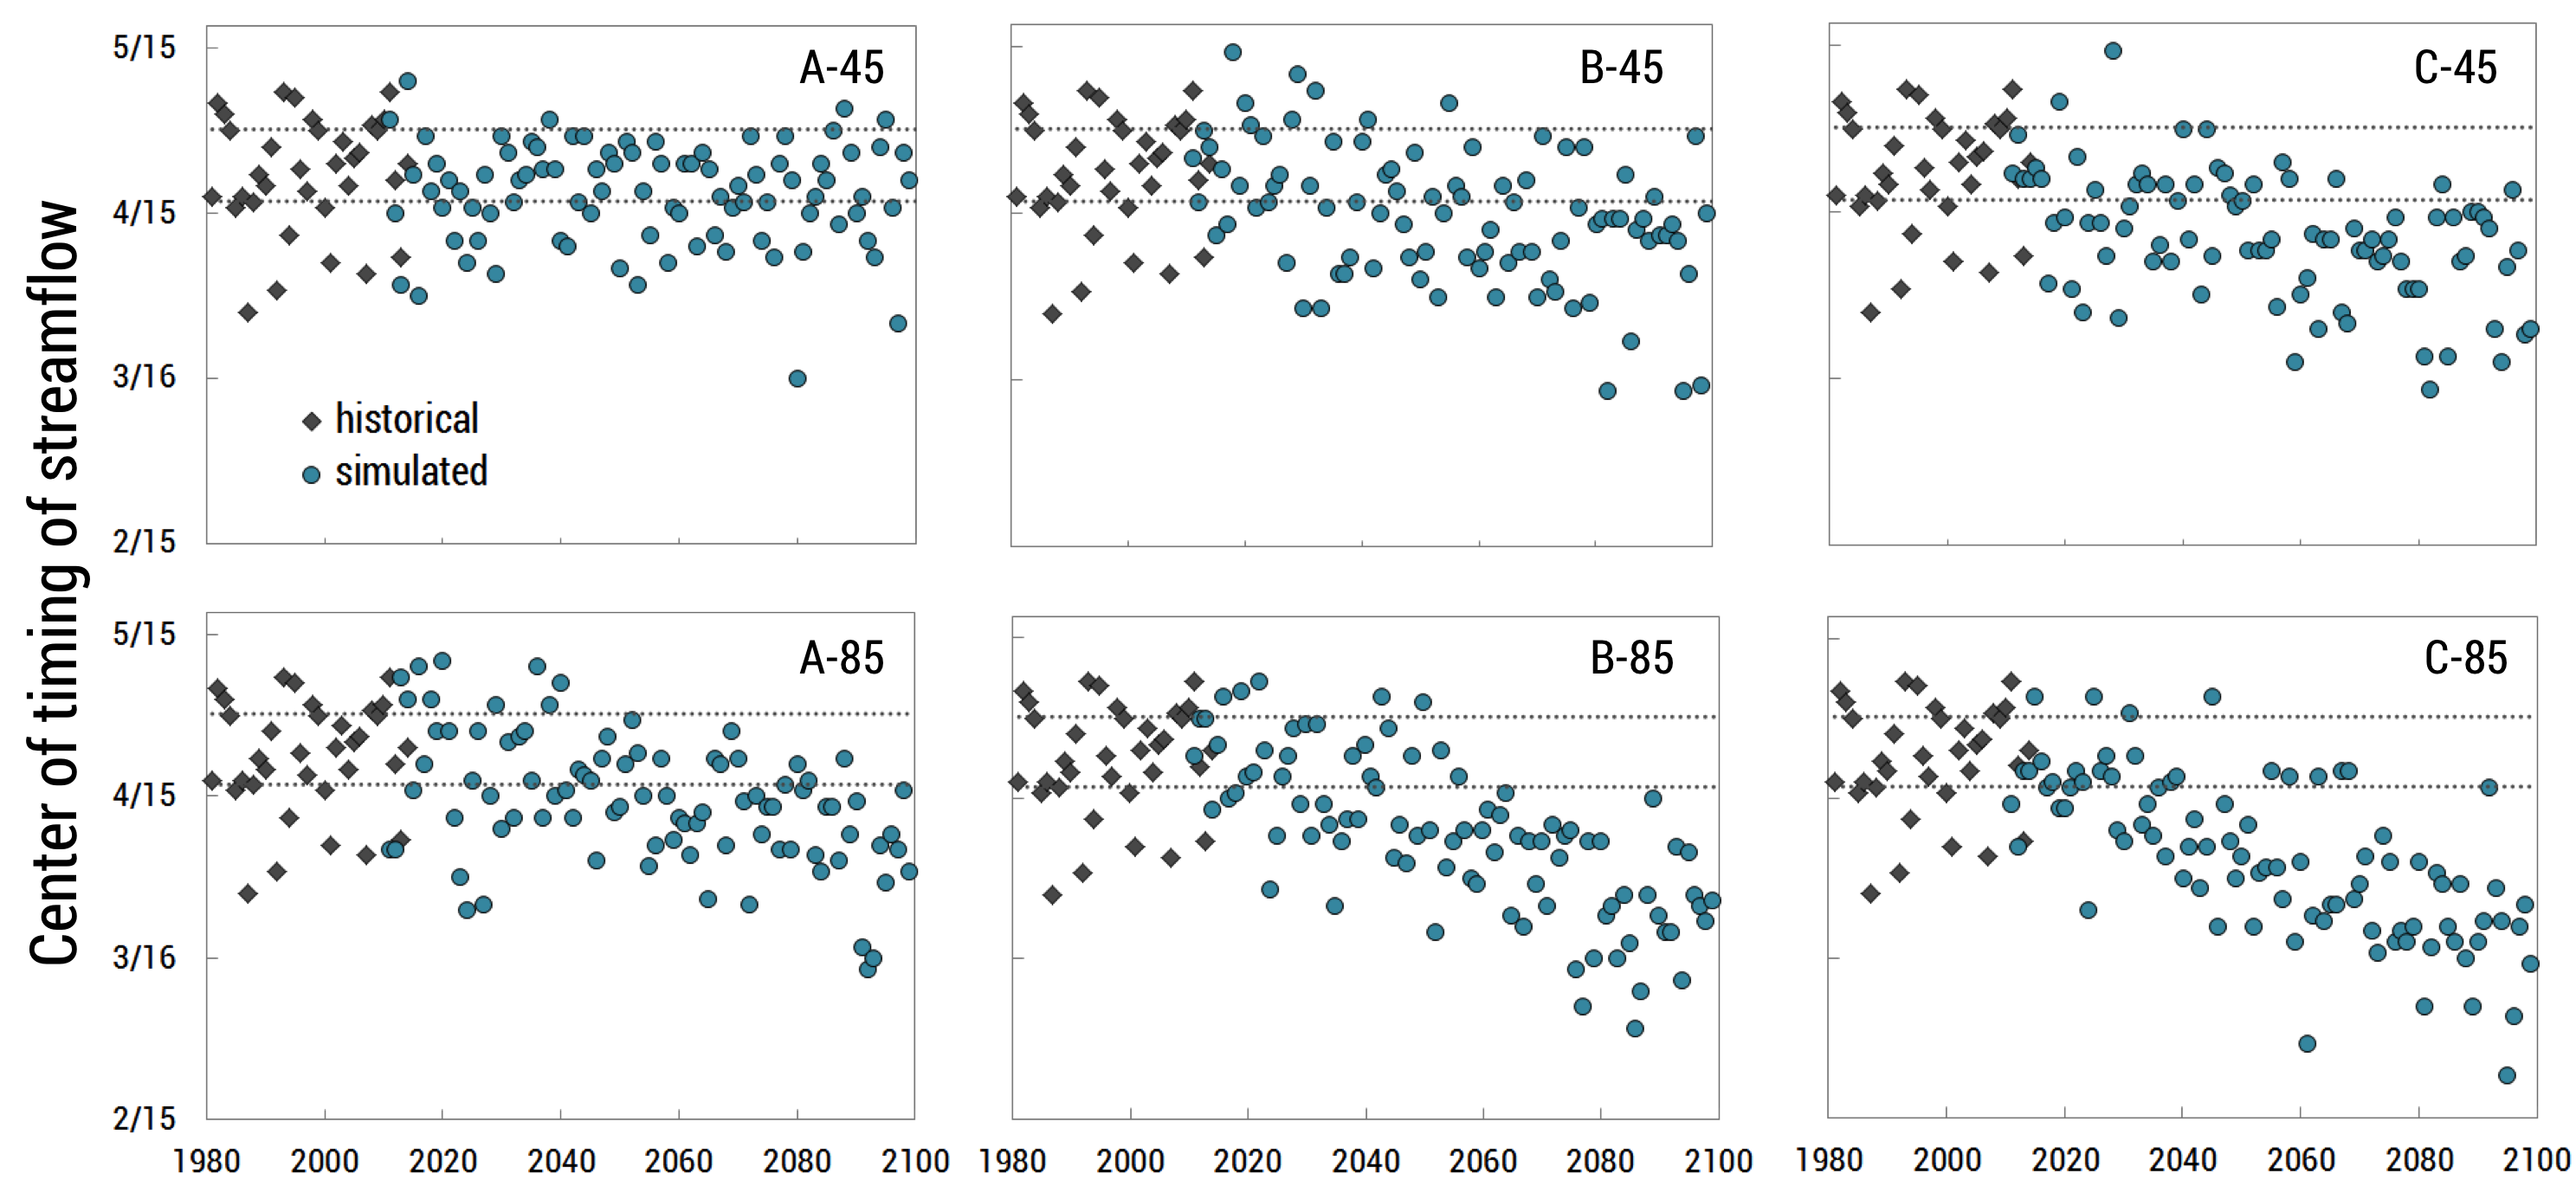
\includegraphics[width=\textwidth]{figure-files/figure11.png}
\caption{Center of timing of streamflow for historic and future simulations. Dashed lines show the upper and lower quartile ranges from 1980-2009. }
\label{fig:CenterOfTiming}
\end{figure}
\clearpage

\begin{figure}
\centering
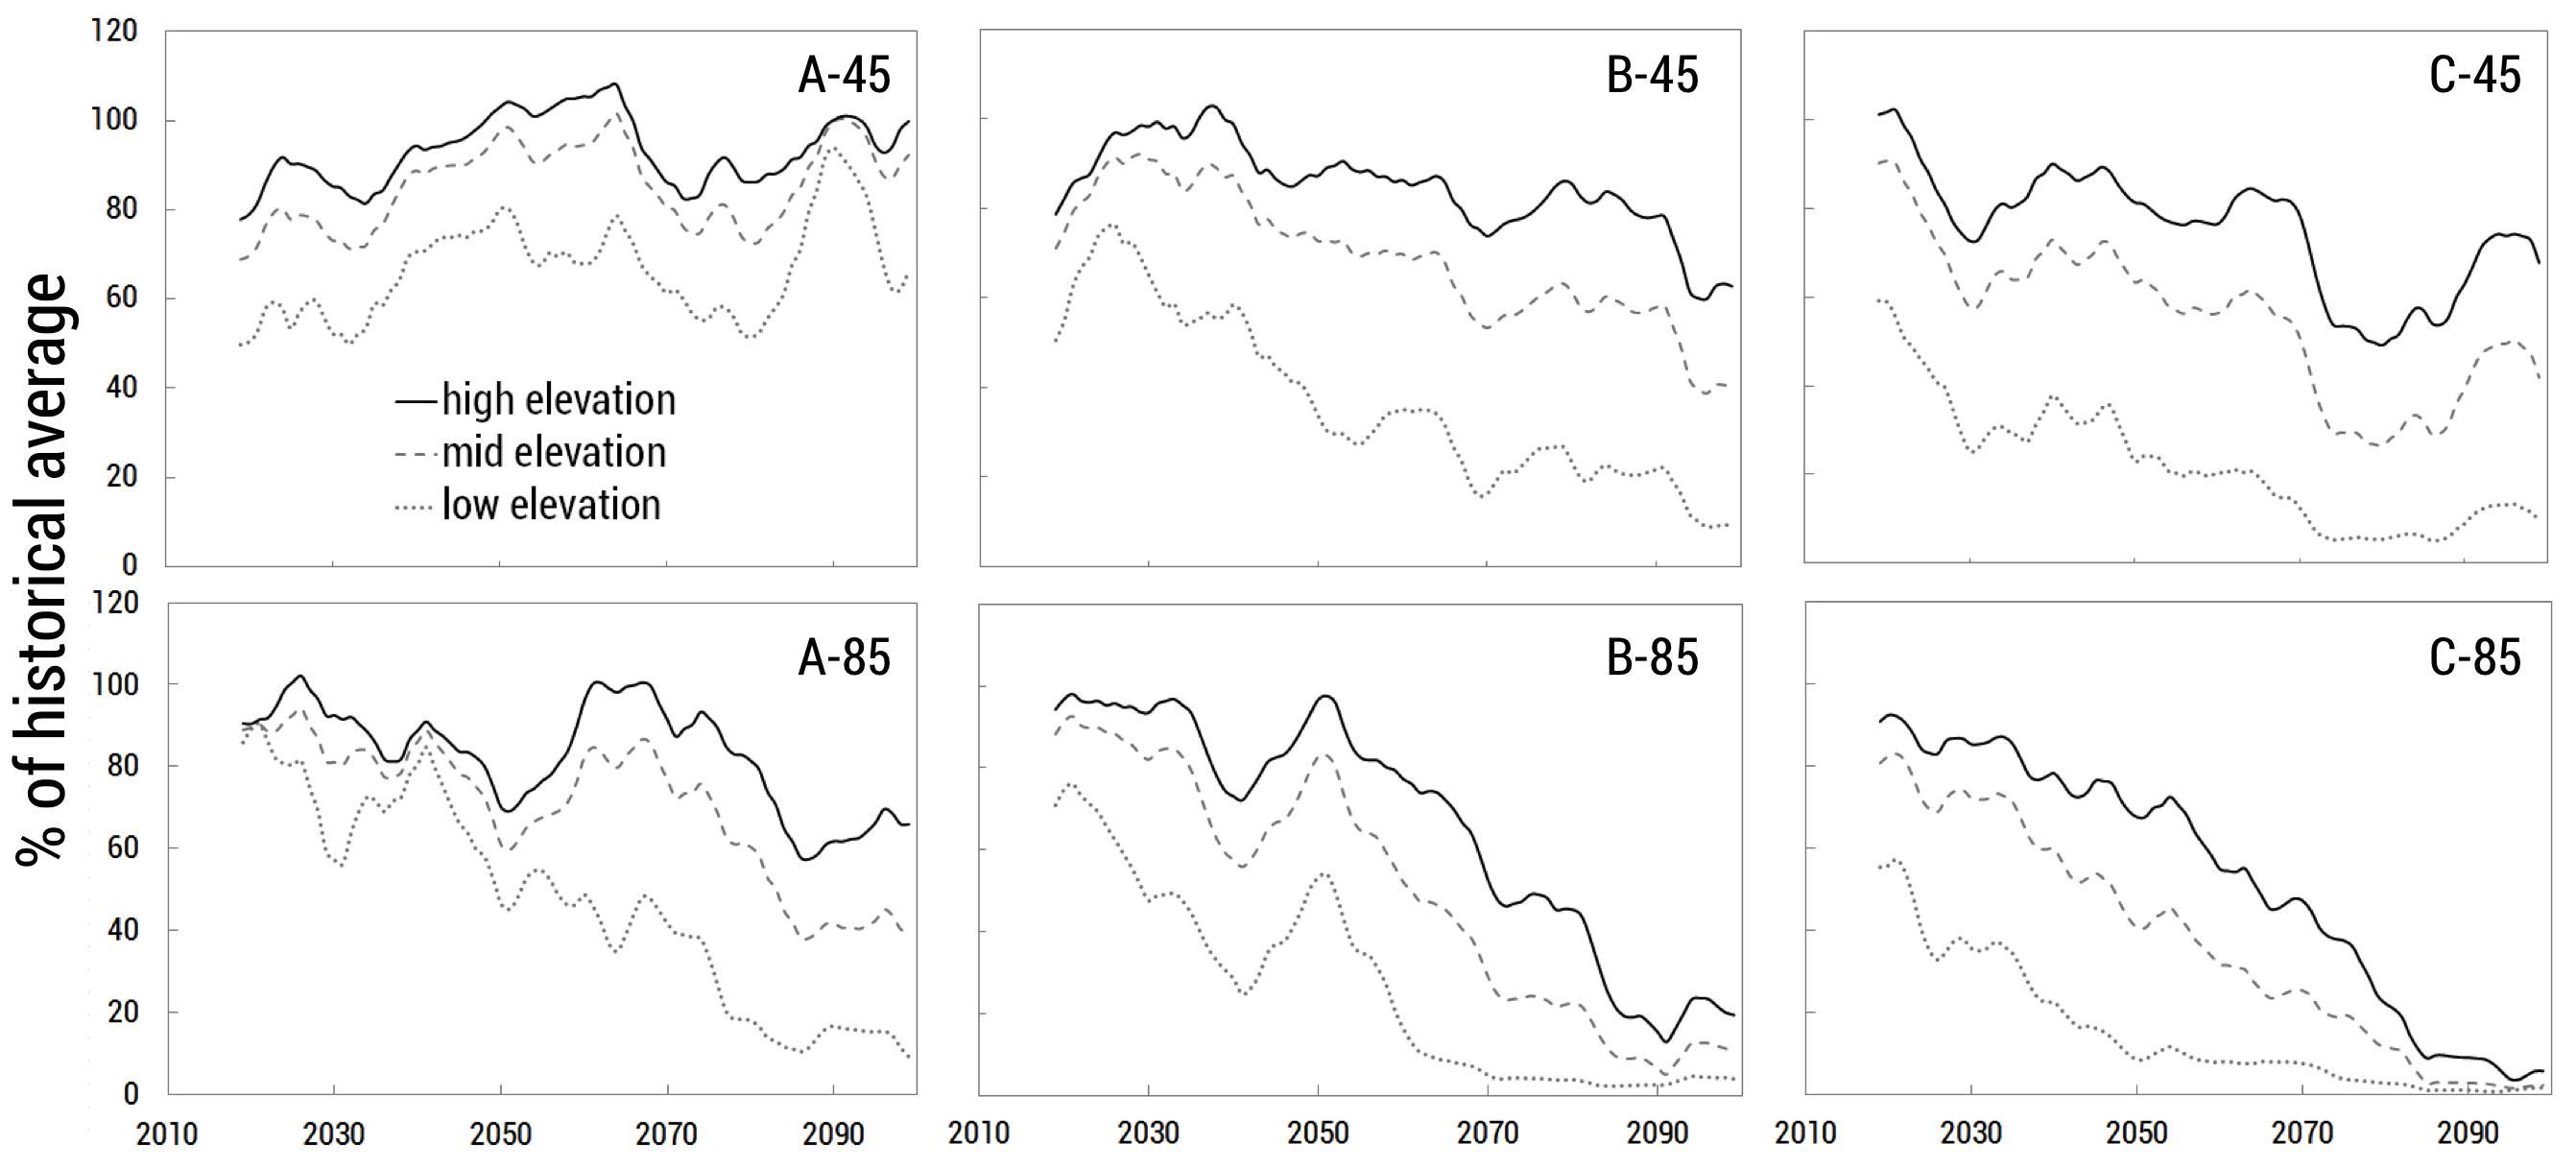
\includegraphics[width=\textwidth]{figure-files/figure12.png}
\caption{10-year moving average percentage of April 1 SWE from historical simulated averages (1980-2009) for low, medium, and high elevation zones, corresponding to 1500-2000, 2000-2500, and 2500+ m, respectively.}
\label{fig:PercentApril1SWE}
\end{figure}
\clearpage

\begin{figure}
\centering
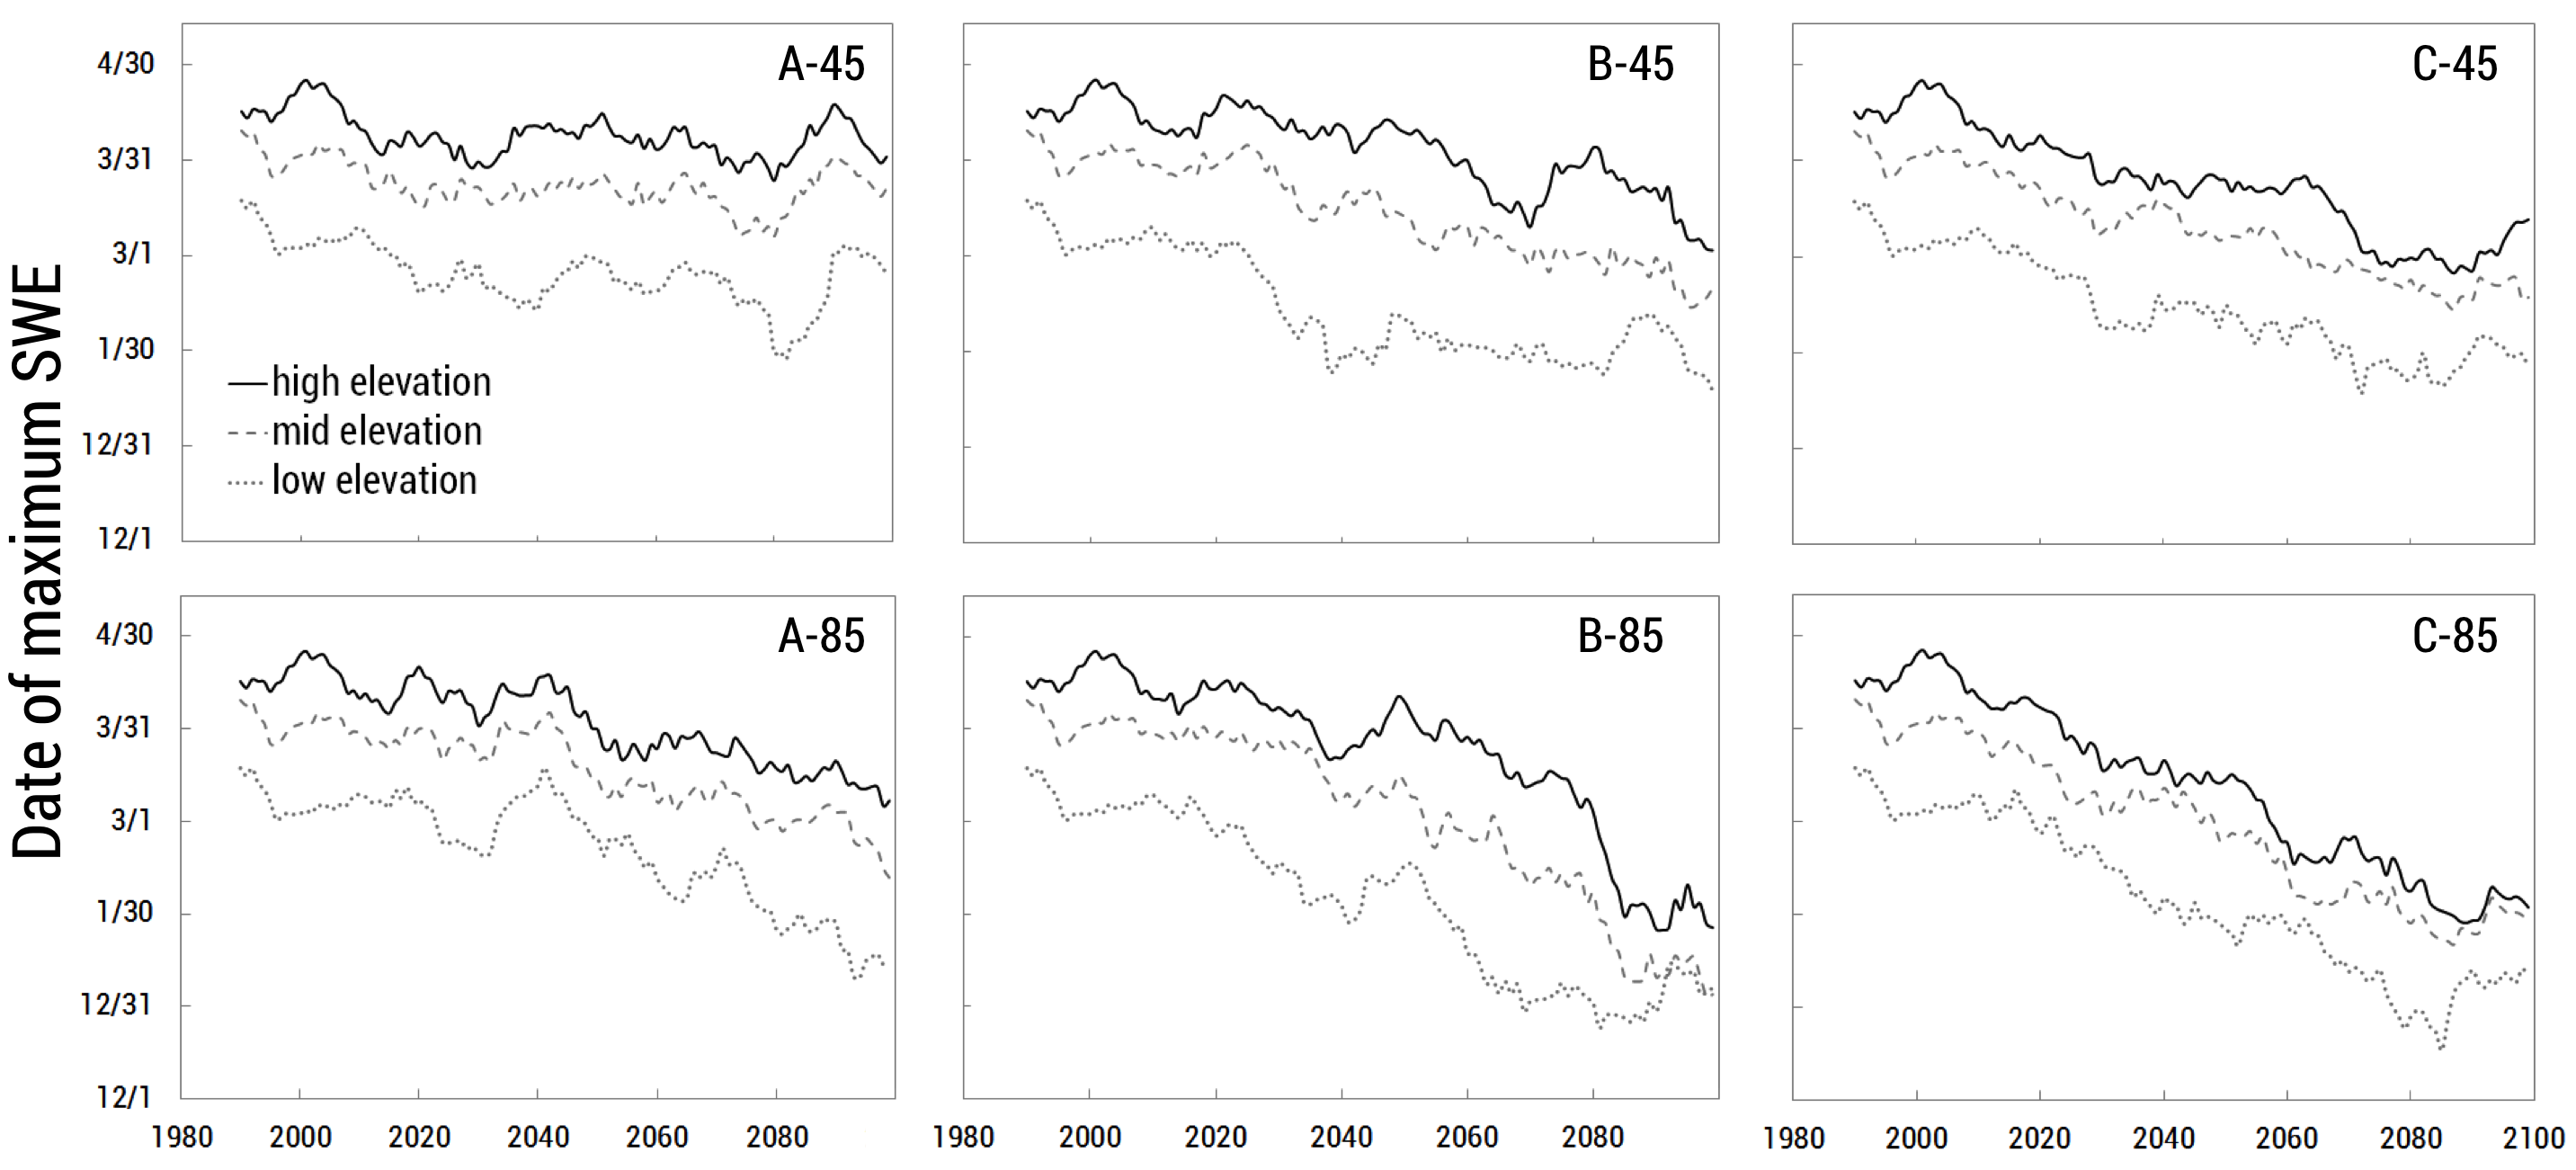
\includegraphics[width=\textwidth]{figure-files/figure13.png}
\caption{10-year moving average of dates of maximum SWE for three elevation zones. Values for 1980-2009 are simulated with MACA METDATA.}
\label{fig:MaxSWEDate}
\end{figure}
\clearpage

\begin{figure}
\centering
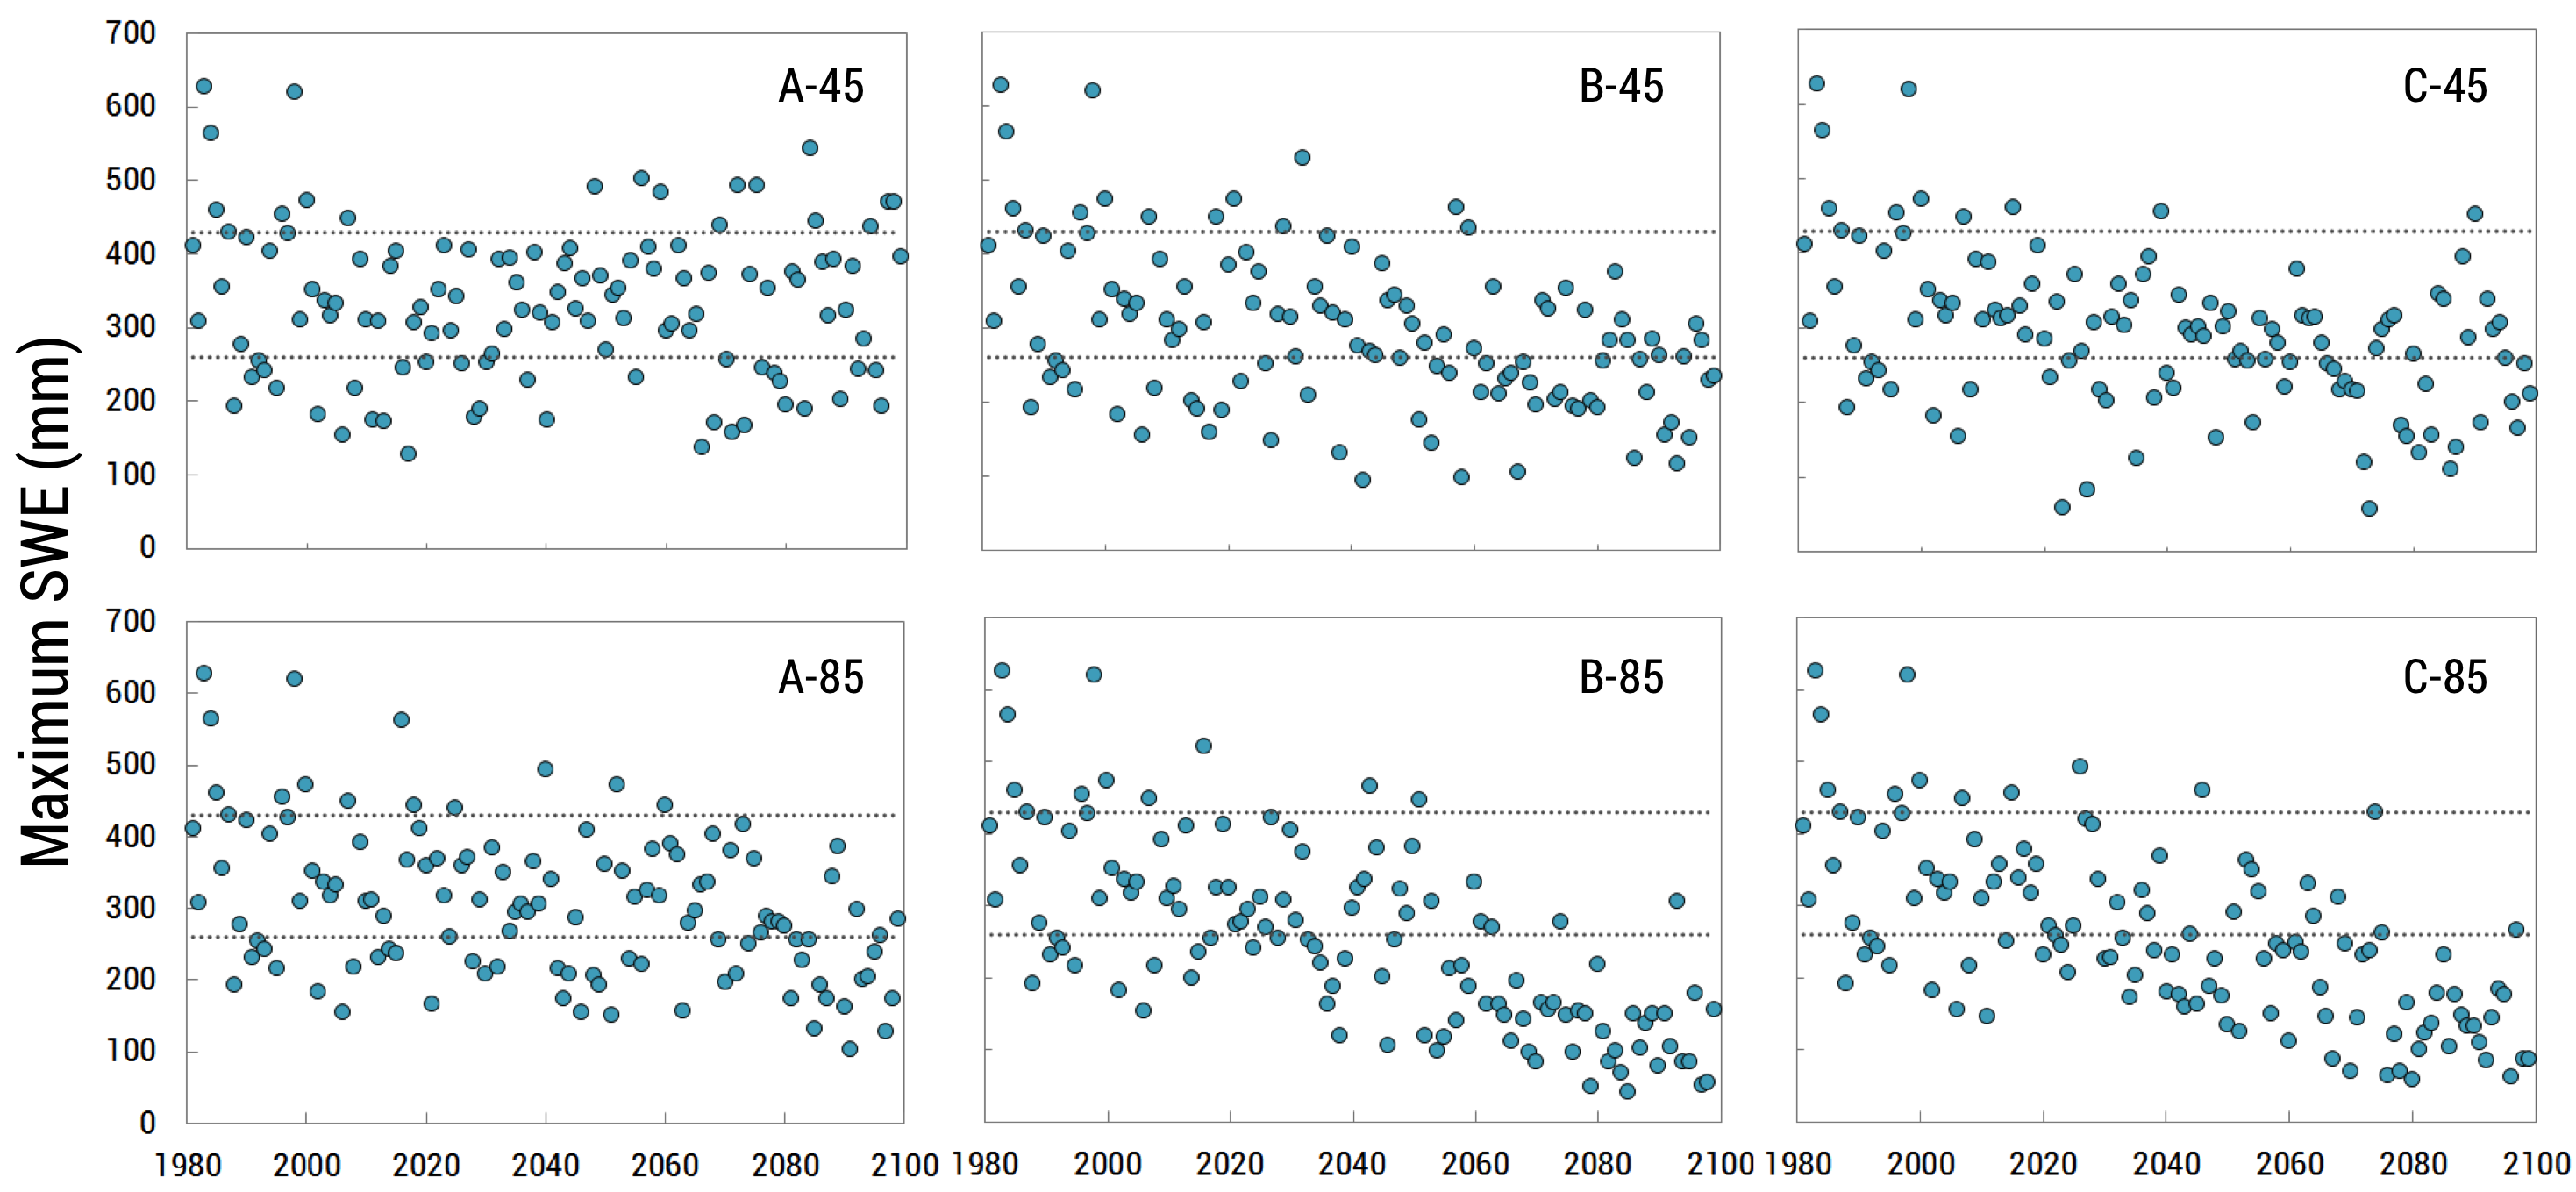
\includegraphics[width=\textwidth]{figure-files/figure14.png}
\caption{Maximum SWE amount (mm) for mid-elevations (2000-2500 m). Values for 1980-2009 are simulated with MACA METDATA. Dashed lines show upper and lower quartile ranges for 1980-2009.}
\label{fig:MaxSWEMidElev}
\end{figure}
\clearpage

\begin{figure}
\centering
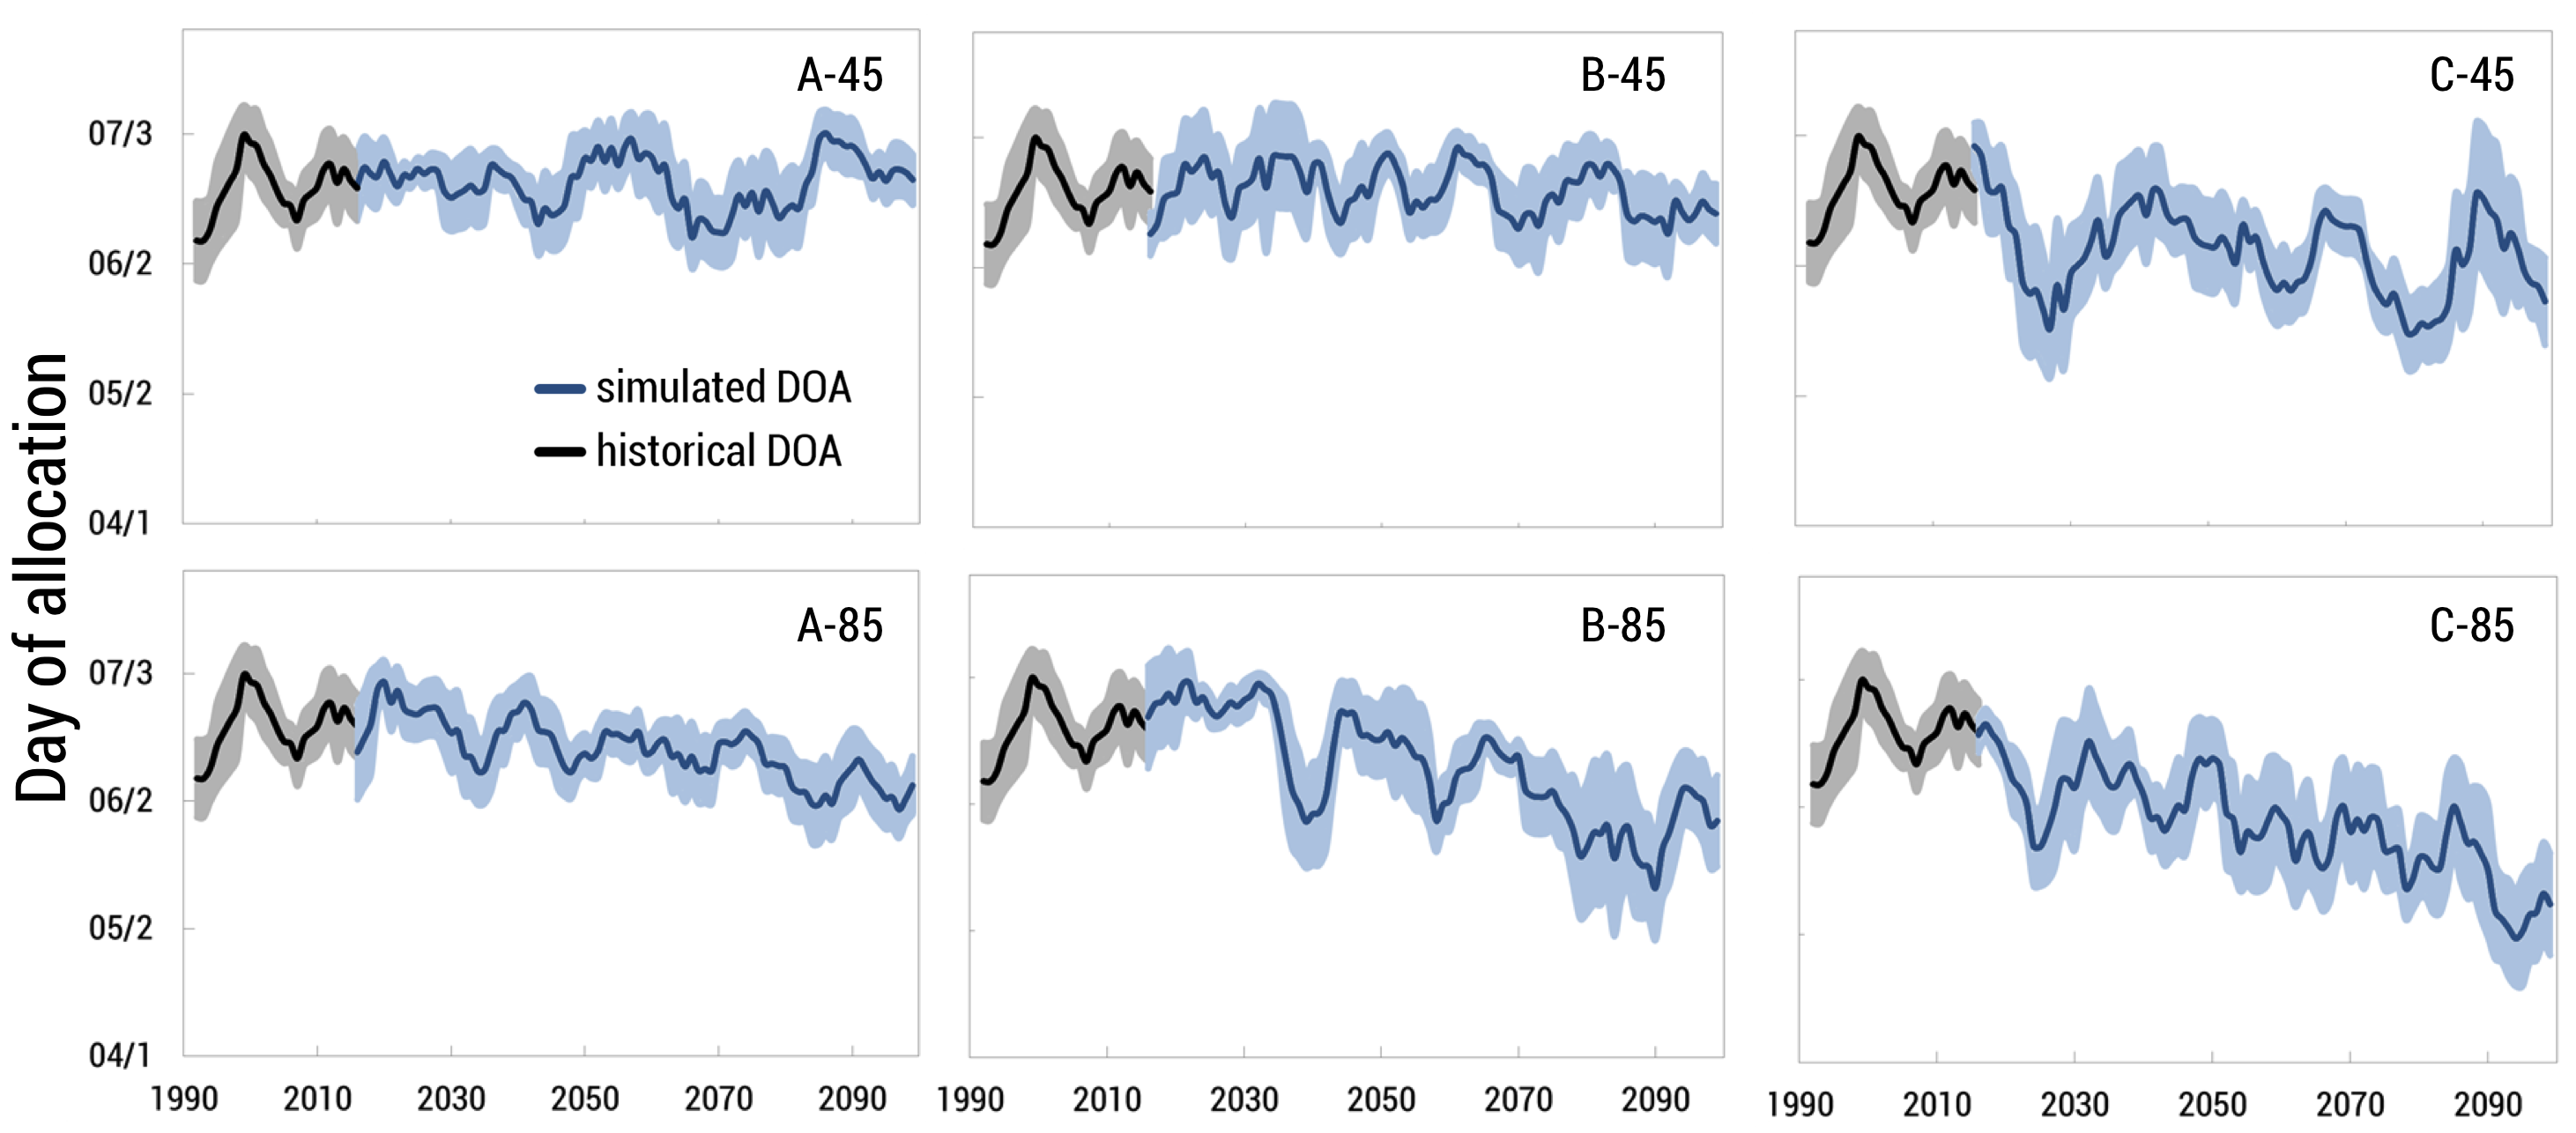
\includegraphics[width=\textwidth]{figure-files/figure15.png}
\caption{Simulated future (2010-2099) and historical (1986-2014) Day of Allocation with a 7-year moving average. Shaded area is $\pm 0.5\sigma$ of 7-year moving average values.}
\label{fig:FutureDayOfAllocation}
\end{figure}
\clearpage

%%f
%\begin{figure}[t]
%\includegraphics[width=8.3cm]{FILE NAME}
%\caption{TEXT}
%\end{figure}
%
%%% TWO-COLUMN FIGURES
%
%%f
%\begin{figure*}[t]
%\includegraphics[width=12cm]{FILE NAME}
%\caption{TEXT}
%\end{figure*}
%
%
%%% TABLES
%%%
\begin{table}
\caption{Data sources used for spatial coverage in Envision}
\label{table:DataSources}
\centering
\begin{tabular}{l l l}
\hline\hline
Input Data (\textit{resolution}) & Data Sources & Used In\\
\hline
Surface Management Agency & Bureau of Land Management & IDU \\
Land Cover (30 m) & National Landcover Database (2011) & IDU, ET \\
Streams \& Catchments (HUC12) & NHD Plus V2 & IDU, HBV \\
Elevation (30 m) & National Elevation Dataset & HRU \\
\hline\hline
\end{tabular}
\end{table}
\clearpage

\begin{table}
\caption{Land cover type in Envision and the associated crop used to calculate evapotranspiration}
\label{table:LandCoverType}
\centering
\begin{tabular}{l l l}
\hline\hline
Land Cover & Crop substituted for land cover & Source \\
\hline
Forest & 3${}^{\mathrm{rd}}$ year poplar $\times$ 3 & Agrimet, \citet{Inouye:2014ws} \\
Shrubland & Sagebrush & \citet{Allen:2007ta} \\
Grassland & Bunch grass & \citet{Allen:2007ta} \\
Wetlands & Poplar $\times$ 3 & Agrimet, \citet{Inouye:2014ws} \\
Developed & Lawn $\times$ 0.21 & Agrimet, \citet{Inouye:2014ws} \\
Agricultural & Alfalfa (mean) & Agrimet \\
\hline\hline
\end{tabular}
\end{table}
\clearpage

\begin{table}
\caption{Naming convention for the six climate scenarios used in this study}
\label{table:ExperimentDesign}
\centering
\begin{tabular}{c c c c}
\hline\hline
 & GFDL-ESM2M & CNRM-CM5 & CanESM2 \\
 & (warm) & (warmer) & (warmest) \\
\hline
RCP4.5 & A-45 & B-45 & C-45 \\
RCP8.5 & A-85 & B-85 & C-85 \\
\hline
\hline
\end{tabular}
\end{table}
\clearpage

\begin{table}
\caption{Parameters for Flow and the ranges/values considered for calibration}
\label{table:FlowParams}
\centering
\begin{adjustbox}{angle=90}
\begin{tabular}{p{1.25in} p{0.75in} p{1.5in} p{1in} p{1in} p{0.75in}}
\hline\hline
Routine & Parameter & Description & Units & Range & Value \\
\hline
\multirow{7}{*}{\parbox{1.25in}{Snow Routine}} & TT & Threshold temperature & ${}^{\circ}$C & -0.5 -- 2.0 & 1.335 \\
 & CFMAX & Degree-day factor & mm${}^{\circ}$C${}^{-1}$ day${}^{-1}$ & 1.0 -- 6.0 & 1.489 \\
 & SFCF & Snowfall correction factor & - & 0.7 -- 1.2 & 0.568 \\
 & CFR & Refreeze coefficient & - & - & 0.05 \\
 & CWH & Water holding capacity of snowpack & - & - & 0.1 \\
\hline
\multirow{7}{*}{\parbox{1.25in}{Soil and Evaporation Routine}} & FC${}^\ast$ & Max depth of water in soil water reservoir & mm & - & 399.7 \\
 & LP${}^\ast$ & Soil moisture value where actual ET=PET & mm & - & 247.2 \\
 & WP${}^\ast$ & Wilting point in soil for ET to occur & mm & - & 156.2 \\
 & BETA & Shaping coefficient & - & 1.0 -- 6.0 & 2.015 \\
\hline
\multirow{6}{*}{\parbox{1.25in}{Groundwater and Response Routine}} & PERC & Percolation coefficient & day${}^{-1}$ & 0.1 -- 2.0 & 1.272 \\
 & UZL & Threshold for K0 to outflow & mm & 1.0 -- 400.0 & 365.4 \\
 & K0 & Recession coefficient & day${}^{-1}$ & 0.1 -- 1.0 & 0.339 \\
 & K1 & Recession coefficient & day${}^{-1}$ & 0.01 -- 0.5 & 0.079 \\
 & K2 & Recession coefficient & day${}^{-1}$ & 0.001 -- 0.15 & 0.004 \\
\hline
\hline
\multicolumn{6}{l}{${}^\ast$ values obtained from ORNL DAAC SDAT} \\
\end{tabular}
\end{adjustbox}
\end{table}
\clearpage

\begin{table}
\caption{Data sites used for calibration and validation. See Figure \ref{fig:StudySite} for locations of gauges.}
\label{table:CalValData}
\centering
\begin{tabular}{>{\centering\arraybackslash}m{0.3in} p{2.5in} >{\centering\arraybackslash}m{1in} p{1in} >{\centering\arraybackslash}m{1in}}
\hline\hline
\centering Type & \centering Name & \centering Drainage Area (km${}^2$) & \centering Record Length & Site ID \\
\hline
\multirow{4}{*}{\centering\begin{sideways}Gauge\end{sideways}} & a) Boise River nr Twin Springs & 2154.9 & 1911 -- present & 13185000 \\
 & b) SF Boise River nr Featherville & 1660.2 & 1945 -- present & 13186000 \\
 & c) Mores Creek abv Robie Creek & 1028.2 & 1950 -- present & 13200000 \\
 & d) Boise River at Lucky Peak${}^\ast$ & 6571 & 1895 -- present & LUC \\
\hline\hline
\centering Type & \centering Name & \centering Elevation (m) & \centering Record Length & Site ID \\
\hline
\multirow{9}{*}{\centering\begin{sideways}SNOTEL\end{sideways}} & Atlanta Summit & 2310 & 1981 -- present & 306 \\
 & Camas Creek & 1740 & 1992 -- present & 382 \\
 & Dollarhide Summit & 2566 & 1981 -- present & 450 \\
 & Graham Guard Station & 1734 & 1981 -- present & 496 \\
 & Jackson Peak & 2155 & 1981 -- present & 550 \\
 & Mores Creek & 1859 & 1981 -- present & 637 \\
 & Prairie & 1463 & 1987 -- present & 704 \\
 & Trinity & 2368 & 1981 -- present & 830 \\
 & Vienna Mine & 2731 & 1979 -- present & 845 \\
\hline
\hline
\multicolumn{5}{p{\linewidth}}{${}^\ast$not an actual gauge, but a calculated daily average of runoff at this location if dams were not present. Obtained from the US Bureau of Reclamation.} \\
\end{tabular}
\end{table}
\clearpage

\begin{table}
\caption{Calibration and validation results for the chosen parameter set for this study.}
\label{table:CalValValues}
\centering
\begin{tabular}{c c c c c | c c c c c}
\hline\hline
\multicolumn{5}{c}{Calibration} & \multicolumn{5}{c}{Validation} \\
\hline
$NSE_G$ & $\log NSE_G$ & $VE_G$ & $NSE_S$ & $Obj.$ & $NSE_G$ & $\log NSE_G$ & $VE_G$ & $NSE_S$ & $Obj.$ \\
\hline
0.71 & 0.61 & -0.03 & 0.59 & 0.63 & 0.70 & 0.66 & -0.06 & 0.52 & 0.62 \\
\hline
\hline
\end{tabular}
\end{table}
\clearpage

\begin{table}
\caption{Simulated mean Day of Allocation (DOA) and standard deviation (italicized, in parentheses) over three future time intervals. Historical (1986-2014) average DOA is 6/19.}
\label{table:SimulatedDOA}
\centering
\begin{tabular}{c c c c c c c}
\hline\hline
Time Period & A-45 & B-45 & C-45 & A-85 & B-85 & C-85 \\
\hline
2010-2039 & 6/22 (12.0) & 6/21 (20.0) & 6/10 (24.3) & 6/19 (17.1) & 6/20 (20.6) & 6/10 (19.0) \\
2040-2069 & 6/20 (17.3) & 6/20 (15.3) & 6/7 (16.8) & 6/15 (13.1) & 6/15 (17.2) & 5/30 (23.5) \\
2070-2099 & 6/23 (15.1) & 6/18 (16.1) & 5/29 (24.0) & 6/8 (14.9) & 5/27 (25.6) & 5/17 (23.5) \\
\hline
\hline
\end{tabular}
\end{table}
\clearpage

\end{document}
